% Equal margins for pdf, if printing may want a larger left margin 
% for single sided or alternating margins for double
\documentclass[equalmargins,oneside,openany]{ut-thesis}
%equalmargins,oneside,openany

% Preamble contains the various packages used
\usepackage{import}
\usepackage{preamble}
% Drop Cap large letter library
\usepackage{lettrine}
%\usepackage[utf8]{inputenc}
%\usepackage{amsmath,amssymb}

\addbibresource{Bibliography/thesis_bib_2023.bib} % This is my bibliography file
%%%%%%%%%%%%%%%%%%%%%%%%%%%%%%%%%%%%%%%%%%%%%%%%%%%%%%%%%%%%%%%%%%%%%%%%%%%%%%%%
%% Algorithmic
%%%%%%%%%%%%%%%%%%%%%%%%%%%%%%%%%%%%%%%%%%%%%%%%%%%%%%%%%%%%%%%%%%%%%%%%%%%%%%%%

\newcommand*\Let[2]{\State #1 $\gets$ #2}


%%%%%%%%%%%%%%%%%%%%%%%%%%%%%%%%%%%%%%%%%%%%%%%%%%%%%%%%%%%%%%%%%%%%%%%%%%%%%%%%
%% Basic shortcuts
%%%%%%%%%%%%%%%%%%%%%%%%%%%%%%%%%%%%%%%%%%%%%%%%%%%%%%%%%%%%%%%%%%%%%%%%%%%%%%%%

%% Matrices and vectors
\NewDocumentCommand\bbm{}{ \begin{bmatrix} }
\NewDocumentCommand\ebm{}{ \end{bmatrix} }
\NewDocumentCommand\Vector{m}{ \boldsymbol{\mathbf{#1}} }
\NewDocumentCommand\Matrix{m}{ \boldsymbol{\mathbf{#1}} }
\NewDocumentCommand\Transpose{m}{ \left.{#1}\right.^T }
\NewDocumentCommand\ConjugateTranspose{m}{ \left.{#1}\right.^H }
\NewDocumentCommand\Trace{m}{ \mathrm{tr}\left(#1\right) }
\NewDocumentCommand\Determinant{m}{ \mathrm{det}\left(#1\right) }
\NewDocumentCommand\Norm{m}{\left\Vert#1\right\Vert }
\NewDocumentCommand\Diag{m}{ \mathrm{diag} \left\{ #1 \right\} }

%% Calculus
\NewDocumentCommand\dd{}{ \mathop{}\!\mathrm{d} }
\NewDocumentCommand\PartialDerivative{mm}{ \frac{\partial #1}{\partial #2} }
\NewDocumentCommand\OrdinaryDerivative{mm}{ \frac{\dd #1}{\dd #2} }
%% Optimization
\NewDocumentCommand\ArgMax{m}{ \operatorname*{argmax}_{#1} }
\NewDocumentCommand\ArgMin{m}{ \operatorname*{argmin}_{#1} }

%% Sets
\NewDocumentCommand\Set{m}{ \left\{#1\right\} }
\NewDocumentCommand\Real{}{ \mathbb{R} }
\NewDocumentCommand\Complex{}{ \mathbb{C} }

%% Lie groups and Lie algebras
\NewDocumentCommand\LieGroupSO{m}{ \mathrm{SO}(#1) }
\NewDocumentCommand\LieAlgebraSO{m}{ \mathfrak{so}(#1) }
\NewDocumentCommand\LieGroupSE{m}{ \mathrm{SE}(#1) }
\NewDocumentCommand\LieAlgebraSE{m}{ \mathfrak{se}(#1) }
\NewDocumentCommand\LieGroupSim{m}{ \mathrm{Sim}(#1) }
\NewDocumentCommand\LieAlgebraSim{m}{ \mathfrak{sim}(#1) }
\NewDocumentCommand\LieGroupAdjoint{m}{ \mathrm{Ad}\left(#1\right) }
\NewDocumentCommand\LieAlgebraAdjoint{m}{ \mathrm{ad}\left(#1\right) }

%% Statistics and stochastic processes
\NewDocumentCommand\Expectation{m}{ \mathbb{E}\left[#1\right] }
\NewDocumentCommand\NormalDistribution{mm}{ \mathcal{N}\left(#1,#2\right) }
\NewDocumentCommand\GaussianProcess{mm}{ \mathcal{GP}\left(#1,#2\right) }

%% Miscellaneous
\NewDocumentCommand\AbsoluteValue{m}{ \left\vert#1\right\vert }

%%%%%%%%%%%%%%%%%%%%%%%%%%%%%%%%%%%%%%%%%%%%%%%%%%%%%%%%%%%%%%%%%%%%%%%%%%%%%%%%
%% UTIAS Notation
%%%%%%%%%%%%%%%%%%%%%%%%%%%%%%%%%%%%%%%%%%%%%%%%%%%%%%%%%%%%%%%%%%%%%%%%%%%%%%%%

%% Zero and Identity matrices
\NewDocumentCommand\ZeroMatrix{}{ \Matrix{0} }
\NewDocumentCommand\IdentityMatrix{}{ \Matrix{1} }

%% Coordinate frames and transformations
\NewDocumentCommand\CoordinateFrame{m}{ \underrightarrow{\Matrix{\mathcal{F}}}_{#1} }
\NewDocumentCommand\Rotation{}{ \Matrix{C} }
\NewDocumentCommand\RotationVector{}{ \Vector{\phi} }
\NewDocumentCommand\Transform{}{ \Matrix{T} }
\NewDocumentCommand\TransformVector{}{ \Vector{\xi} }

%% Variable decorations
\NewDocumentCommand\Estimate{m}{\hat{#1}}
\NewDocumentCommand\Prior{m}{\check{#1}}
\NewDocumentCommand\Mean{m}{\overline{#1}}
\NewDocumentCommand\Optimal{m}{{#1}^*}

%%%%%%%%%%%%%%%%%%%%%%%%%%%%%%%%%%%%%%%%%%%%%%%%%%%%%%%%%%%%%%%%%%%%%%%%%%%%%%%%
%% Additional definitions for your document
%%%%%%%%%%%%%%%%%%%%%%%%%%%%%%%%%%%%%%%%%%%%%%%%%%%%%%%%%%%%%%%%%%%%%%%%%%%%%%%%

\NewDocumentCommand\se{m}{ \bm{\mathrm{#1}} }
\NewDocumentCommand\sev{m}{ \vec{\bm{\mathrm{#1}}} }
\NewDocumentCommand\ses{mm}{ \bm{\mathrm{#1}}_{#2} }
\NewDocumentCommand\sesh{mm}{ \hat{\bm{\mathrm{#1}}}_{#2} }
\NewDocumentCommand\sesc{mm}{ \check{\bm{\mathrm{#1}}}_{#2} }
\NewDocumentCommand\sesb{mm}{ \bar{\bm{\mathrm{#1}}}_{#2} }
\NewDocumentCommand\sel{mm}{ \bm{\mathrm{#1}}_{#2}^l }
\NewDocumentCommand\sen{mmm}{ \bm{\mathrm{#1}}_{#2}^{#3} }
\NewDocumentCommand\xtan{m}{ x_l-\check{x}_k-d\cos\check{\theta}_k }
\NewDocumentCommand\ytan{m}{ y_l-\check{y}_k-d\sin\check{\theta}_k }
\NewDocumentCommand\pder{mmm}{ \frac{\partial #1}{\partial #2}\Bigr|_{#3} }
\NewDocumentCommand\pdern{mm}{ \frac{\partial #1}{\partial #2} }
\NewDocumentCommand\siv{m}{ \sigma_v^2 }
\NewDocumentCommand\sio{m}{ \sigma_\omega^2 }
\NewDocumentCommand\sir{m}{ \sigma_r^2 }
\NewDocumentCommand\sip{m}{ \sigma_\phi^2 }










% *******************Title Parameters*******************
\author{Willard Farmer}
\title{The Creation of a New Payload Operations Planning Software} 
\graddegree{Master of Applied Science}
\department{Institute for Aerospace Studies}
\gradyear{2023}

% Load acronymns from seperate tex file
\makenoidxglossaries{}
\loadglsentries{Front Matter/acronym}

% ******************Front Matter*******************
\begin{document}
\frontmatter % 10 pgs

    \maketitle
    \begin{abstract}
    %\doublespacing
	\doublespacing 

As small spacecraft become more capable, so too does the complexity of their
operations. Searching for potential concurrent observation or access
opportunities and ensuring they are compatible with one another may become
tedious and repetitive for operators to manually compute. Currently available
commercial-off-the-shelf tools that automate this process are capable but
expensive. To address this problem, a new payload operations planning tool has
been developed by the Space Flight Laboratory to handle the deterministic
aspects of mission planning, such as: detecting observation opportunities,
validating observations in a schedule, and generating lists of commands to be
sent to satellites. This lightweight tool is generalizable to any
Earth-observing mission configuration, and can support complicated observation
geometries. Open-source libraries were used to reduce the overhead for
development as they decrease the amount of code that must be newly created and
maintained. Functionality has been compartmentalized through a containerized
service-based architecture. In this way, new functionality can be added or
replaced as needed. To enhance usability, a user may interact with the tool
through a browser-based user interface. This thesis outlines the features of the
Payload Operations Planning Software, as well as details about its architecture
and development.

\doublespacing

    \end{abstract}
    
    \begin{acknowledgements}
	There are too many people to name that have either directly or indirectly
contributed to this thesis. 

First, I would like to extend my deepest thanks to my supervisor, Dr. Robert
Zee. His direct and indirect leadership has pushed me to become a better
engineer. His advice and guidance has helped me expand my perspective on what
constitutes a good engineering solution to a problem. I am fortunate to be part
the environment that he has created at the Space Flight Laboratory which serves
as an incubator for the next generation of space engineers.  Thank you for
seeing my potential and giving me the opportunity to push my boundaries and
thrive.

I would next like to thank my mission manager Nathan Cole. I always felt as
though Nathan made myself and the other students working under him a priority.
He would always have time to discuss any problem and ensured that my work was
not only productive and useful to the mission but also thoroughly enriching.
With Nathan, I would also like to thank the other members of the POPS team:
Matt, Lukasz, and Erica. This thesis was made possible through your
collaboration, patience, and advice.  

To my friends, you have made this master's program not only possible but two of
the best years of my life. To my cohort: Diana, Andreas, Lukasz, Djordje, Kim,
Connor, Hooman, Arjun, Eric, and Jacob, I have enjoyed every moment learning
and sharing this experience with you. I know you will all excel wherever you
go. To Jordy, since we met on the first day of second year of undergrad, you
have been a constant companion. Thank you for your patience, support, and
friendship. To Mia, thank you for showing me what is possible through talent,
grit, and determination. Your example has pushed me to work harder and be
better.  To my friends from home: Momo, Julie, Ethan, Saymon, Gurjeet, Mazzen,
and Daylen, thank you for helping me keep my sense of community. Your
friendship has served as my bedrock. 

Oftentimes omitted in academics is physical exercise. I would like to thank the
members of the Swole Patrol: Nathan, Rami, Suraj, and Matt. Through mentorship
and example, they have taught me how to make very heavy things feel less heavy.

Lastly and the most importantly of all, I would like to thank Mum and Dad. I
find it difficult to put into words the appreciation I have for your
unconditional support. It feels as though you're always there, always know
what's best and always know what to do. Team Farmer.


    \end{acknowledgements}
    
    \tableofcontents
    \listoffigures
    \listoftables
   % \listofequations
    \printnoidxglossary[type =\acronymtype, title=List of Acronyms]
    \cleardoublepage{}
	
% ******************Main Body*******************
\mainmatter{}
\glsresetall{} 
\chapter{Introduction}
%\subsection{Small Satellites and New Space}


\section{Thesis Overview}


\lettrine[lines=2, findent=0pt, nindent=5pt]{O}{} ver the past decade, there
has been a sharp rise in the development of small spacecraft. With 112
nanosatellites launched in 2012 and 1800 launched in 20221, it is clear that
the industry is growing. As technology improves, so too do the capabilities of
small spacecraft. For missions with relatively ‘simple’ operations, it is
economical to use competent engineers to handle orbit operations. But, as
missions become more complex, more of the operator’s time is spent on repeated
calculations using purpose-built scripts that offer little in terms of
reusability. For suitably complicated operations, the economy of human
computation is lost. In this scenario, the benefits of software automation
become appealing. Commercial-off-the-shelf tools do exist to address this
issue. A ready example would be Orbit Logic’s \gls{cpaw}2 or their Scheduler
extension for the Ansys \gls{stk}3. These solutions are well-developed and have
a proven mission heritage. They are also quite expensive and still require
adapting to a specific mission scenario.  \\ 


At the \gls{sfl}, the \gls{pops} is being developed to streamline operations
planning for remote sensing missions. \gls{pops} is a general offline software
meant to handle the deterministic aspects of mission planning.  Given an
\gls{aoi} and a method of remote sensing, \gls{pops} presents possible
observation opportunities to the operator and creates sets of commands to be
uploaded to a spacecraft in orbit.  Ideally, \gls{pops} should prevent an
operator from having to do any calculations themselves manually. Not only is
\gls{pops} meant to be a tool used by \gls{sfl} operators but one of the goals
of this project is to reduce the barrier to development as much as possible.
The easier the underlying code is to work with, the more likely it is that
future developers work on it and the tool grows. For this reason, most of the
underlying code for \gls{pops} has been written in Python and leverages several
open-source libraries.  Extending this principle, \gls{pops} uses a
browser-based \gls{gui} rather than as an executable desktop application. As a
browser-based application, \gls{pops} can leverage an extensive set of existing
libraries for building functionality.  For example, CesiumJS4 may be used for
graphical Earth visualizations.  \gls{pops}’s architecture is containerized for
easy deployment, using Docker5.  Each service handles separate aspects of the
software’s functionality.  In this way, they can be developed separately and
switched out as needed. With services, functionality may also be integrated
into other applications. For persistent storage of planning information, an SQL
database has been implemented as its own service.  To facilitate searching for
observation opportunities, a suite of software tools has been developed, known
as the \gls{atu}.  \gls{pops} also handles its orbital propagation by making use of
open-source Python implementations of the SGP4 algorithm. 



\subsection*{Thesis Outline} 


\section{Existing Solutions}\label{sec:exsoln}

This is not a problem that is unique to Gray Jay Pathfinder.
For any mission with sufficiently complicated operations, developing or purchasing a license for planning software is prudent.
There are a multitude of existing solutions, each with their own benefits and shortcomings.




\subsection{\acrshort{cpaw}}

The \gls{cpaw} is the one of the most sophisticated operations planning tools on the market. 
Developed by Orbit Logic, \gls{cpaw} is one of their products available on the open market. 
Others being: SpyMeSat Mobile App, Order Logic, STK Scheduler, UAV Planner, and On-board Autonomous Planning System.
\gls{cpaw} has been used by a number of missions for their imaging planning operations: Landsat 8/9 \cite{gokhale_mission_nodate}, Worldview-1/2, GeoEye-1, and RADARSAT-2 \cite{herz_eo_2014}.


\gls{cpaw} specializes specifically on image planning. 
Once set up by an operator, it can generate operations schedules and can generate commands to be sent to spacecraft in orbit.
It supports both automatic and manual operations.








\glsresetall{} 
\chapter{Operations Concepts}

\lettrine[lines=2, findent=0pt, nindent=5pt]{B}{} efore discussing the
\gls{pops} it is necessary to go over basic terminology.  Without doing so, it
may become very easy for descriptions to become unclear or inprecise.

\section{Definitions}

\begin{description} 

    \item[Area of Interest] An \gls{aoi} is a general concept for some region
	on the Earth that is of some particular importance to a user. It is the
	region which one or more spacecraft should be used to gain more
	information about the area. \glspl{aoi} can be specified as a point
	target, a polygon, or a latitiude range. See section \ref{aoi_def} for
	an exhaustive definition in this context. 

    \item[Field of View] The \gls{fov} is the extent a sensor or instrument may
	observe the outside world at a given time. The size and shape of an
	\gls{fov} varies based on the design of the sensor or instrument in
	question. Unless otherwise specified, for the purposes of this thesis,
	it may be assumed that \glspl{fov} are conical. Specifically, the
	\gls{fov} is defined by a single half-angle, $\theta$. Suppose an
	instrument is pointing along some vector, $\vec{u}$. Let us define
	another vector, $\vec{v}$ such that the angle between it and $\vec{u}$
	is $\theta$. The \gls{fov} is the volume described by rotating
	$\vec{u}$ around $\vec{v}$.

    \item[Field of Regard] The \gls{for} is similar to the \gls{fov}. Instead
	of the area an instrument can observe in a singular time instant, the
	\gls{for} is the area an instrument can possibly observe by changing
	its prientation given an external constraint. It is not possible to
	observe the entire \gls{for}. Rather, only a subset of the \gls{for}
	can be observed. This subset is the instrument's \gls{fov}. For
	example, let us consider an optical sensor fixed to a spacecraft
	orbiting the earth. The position of the sensor at particular time
	instant is given by the spacecraft's orbit and cannot be changed unless
	the spacecraft's orbit is changed. Of course, the position of sensor
	can be changed slightly by changing the attiutde of the spacecraft,
	since the instrument is most likely not located at the spacecraft's
	centre of mass. But, this can be ignored since the distance the
	instrument can translate is negligeable compared to its orbit. The
	orientation of the instrument can be changed, though, and this has a
	meaningful effect on the \gls{for}. If no constraints are put on the
	attitude of the spacecraft, the \gls{for} is everywhere, since the
	instrument can be pointed in any direction. Let us say the spacecraft
	can only point an angle, $\alpha$, off nadir. The \gls{for} would then
	be the cone described by the half-angle $\alpha + \theta$, where theta
	is again the half-angle of the conical sensor. \textbf{(MAKE A NEW
	'EXAMPLE SECTION')}
 

    \item[Footprint] The footprint is the area on Earth that can be observed by
	an instrument's \gls{fov} or \gls{for} at a given time. It can be found
	by intersecting the \gls{fov} or \gls{for} with the surface of the
	Earth.  These intersection points form a boundary and the enclosed area
	within this boundary is the footprint. For clarity, it should be
	assumed that footprint refers to an \gls{for}'s footprint, unless
	otherwise specified.

    \item[Swath] A swath is the union of all footprints over a time range for a
	particular sensor.


    \item[Horizon Swath] A horizon swath is a special case where the entire
	Earth is within the \gls{for}. 




	
\end{description}




\glsresetall{} 
\chapter{Software Architecture}


\section{POPS Architecture}

The \gls{pops} is made up of several distinct components separated into
services.  Each service has its own Docker5 container. Containers are similar
to virtual machines in that they simulate an operating system but, unlike
virtual machines, they do not simulate the underlying hardware. This makes
containers much more lightweight, while also retaining the benefits of having a
standardized environment where dependencies are packaged with their source
code. Containers make deploying and maintaining \gls{pops} much easier since
installation does not require managing dependencies and tweaking environment
variables. In this way, a \gls{pops} user does not need to be as familiar with
the software as a developer to run it. Each service is its own Python web
server.  In this way, they may be interacted with via a RESTful API. That
being, HTTP requests can be made to retrieve information or perform
calculations. Each service also provides its own automatically generated
documentation that can be accessed through a web browser. This documentation
outlines possible API calls as well as their input and output data formats.
This allows a user to quickly see the capabilities of a service without
accessing the source code. Currently, \gls{pops} has 4 main services; they are
the: Mission Model, Propagator, Database, and Access Time Utilities.  Mission
Model.


\subsection{Mission Model}

The Mission Model service is the service that contains the main logic for most
of \gls{pops}’s functionality and front-end GUI. When a user interacts with
\gls{pops}, they are interacting with the Mission Model service.   Part of the
Mission Model service supports the 3D Earth visualization tool, CesiumJS4.
CesiumJS can display time-dynamic, geospatial information on a webpage.  With a
custom-made Cesium handler class, \gls{pops} can visualize: the Earth,
spacecraft, their orbits, ground stations, and can draw polygons on the Earth.
In addition to displaying information, the handler class also enables a user to
make changes in the viewer which are then reflected in \gls{pops} itself. The
mission model service has many other features including: database management,
opportunity filtering, and scheduling. These features will be discussed in the
WORKFLOW section.  

\subsection{Propagator}

The Propagator service handles ephemeris generation for \gls{pops}.
Ephemerides are a crucial component for every subsequent step along the
planning process so it is essential that they are well formed. Consolidating
ephemeris generation for the entire tool ensures that only one area of the code
needs to be developed and validated.

Currently, the main method of orbital propagation for \gls{pops} is with the
\gls{sgp} model series of algorithms, specifically SGP4/SDP4 referred to as
just ‘SGP4’. SGP4 is an analytical method of approximating orbital state
vectors at corresponding epochs in the \gls{teme} \gls{eci} coordinate frame,
given a NORAD \gls{tle}.  \gls{tle}s are readily provided by the United States
Space Force through Space-Track6 or CelesTrak7. The \gls{teme} coordinate frame
is not particularly useful so part of the Propagator service’s purpose is
transforming the orbit vectors into a coordinate system required by other parts
of \gls{pops}.  Currently, the two possible output reference frames are the
\gls{gcrs}, which is an \gls{eci} reference frame, and the \gls{wgs}, which is
an \gls{ecef} reference frame.  Depending on the application, it is sometimes
useful to use \gls{eci} or \gls{ecef} reference frames, so both are made
available by the service.  Given a \gls{tle}, a time range, a step size, and a
coordinate system, the Propagator service generates an Ephemeris for the
provided time range in a variety of output formats.

It is very easy to generate Ephemeris data. What is difficult is validating it.
The benchmark for validation is \gls{stk} since it has its own SGP4 ephemeris
generation capabilities. If operators did not use POPS, their best alternative
would be to set up scenarios manually in \gls{stk}. As such, using it as ground
truth is valid in this case. Both \gls{stk} and the \gls{pops} implementation
of SGP4 us the same source8: Revisiting Spacetrack Report \#39. As such, they
should provide the same results. One difference to note is that \gls{stk} uses
the \gls{icrf} \gls{eci} coordinate system but the propagator service uses
\gls{gcrf}.  This difference is acceptable since these reference frames are
approximately identical10. The procedure for validating the Propagator service
was first to select a \gls{tle}, a time range, a time step, and a coordinate
system.  Next was to generate Ephemerides from \gls{stk} and the propagation
service.  Finally, the results were compared. One such comparison can be seen
in Figure \ref{fig:stk_py}. Here, the peak position residual was 0.37mm for the position along
the x-axis. The main purpose of this exercise is to ensure that the Python
libraries are being used correctly and that their output data is acceptable.
From this result, it is clear that the methods are identical and the difference
was most likely due to slight implementation differences. 

\begin{figure} 
    \centering
    \includegraphics[width=0.7\textwidth]{STK_PY_residual-2.png} 
    \caption{Residual Difference \gls{stk} vs. Python}
    \label{fig:stk_py} 
\end{figure}

Part of the benefit of having the Propagator as its own service is that if a
more accurate algorithm is desired for orbital propagation, only the Propagator
service needs to be changed and the rest of \gls{pops} can be left as is.


\subsection{Access Time Utilities}

The ATU service provides the basic building blocks for
constraining observation opportunities. These can be added to depending on a
mission’s need. The \gls{atu} service currently supports calculating: ground station
access times, swath generation, horizon swath generation, and polygon
intersection with a swath. These will be discussed in detail in their own
section.  


\subsection{Database}

\gls{pops} must be able to retain information, even if it is
shut down or moved somewhere else. It is also necessary that data be stored
such that it does not sit in RAM. For this reason, an SQL database service is
included. It stores all the data necessary for \gls{pops} to function. This
includes but is not limited to satellite information, \gls{tle}s, current and
previous plans, ephemeris data, observation opportunity data, and planned
observations. Using an SQL database allows for effective data storage and
access. There are also no read or write restrictions on an SQL database so data
can be accessed simultaneously by multiple users or services.





\section{Access Time Utilities}


The Access Time Utilities are the fundamental components that enable POPS to be
a planning software. They form the basic building blocks for constraining
observation opportunities. Additional utilities can be added depending on a
mission’s need. The following sections discuss the baseline functionality that
has currently been implemented.


\subsection{Ground Access Utility}

A Ground Access is defined as the time interval during which a satellite can
establish contact with a ground station. A ground station is a point on the
Earth’s surface, identified with geodetic latitude-longitude-altitude
coordinates and an elevation mask. An elevation mask is the angle above the
horizon, at the ground station’s position, at which the satellite can be
considered visible by the ground station. Calculating the ground access for
satellites on a mission is a fundamental task in operations planning. These
time intervals dictate the opportunities for data downlink, command uplink, and
any other communication between the ground segment and satellite. 

The simplest way to compute ground access involves propagating the orbit of a
satellite and checking, at every time step, the position of the satellite
relative to the ground station and testing whether the relative position is
above the elevation mask. While this method is trustworthy and capable of
returning accurate results, its reliance on iterating over an entire satellite
orbit input typically yields a long runtime. This is particularly evident in
the case where a mission has multiple ground stations, multiple satellites, or
a short propagator timestep. The computation time drawback motivates the use of
other algorithms that can determine ground access more efficiently. 

There have been a plethora of papers published on the subject of efficiently
computing ground access over the years. Early work includes Lawton’s
development of a method for calculating ground access for low-eccentricity
satellite orbits by leveraging the Fast Fourier Transform to quickly find a
ground access11. Alfano et al.12 use another technique known as parabolic
blending for constructing the visibility function and finding ground access.
While POPS currently utilizes the simplest method for calculating ground
access, the method that is selected for future implementation is that of Han et
al.13, which uses a self-adaptive interpolation technique to approximate the
waveform of the visibility function. The advantage of this method is its
suitability for all orbit types and orbit propagators, which allows the methods
employed by POPS to generalize for any mission orbit definition. 


\subsection{Swath Utility} 

As discussed in the Terminology section, the concept of an access swath is
defined as a time-series of access regions as a satellite orbits the Earth.
Within \gls{pops}, a swath is represented through a closed curve that describes
the boundary of the cumulative access region of a sensor’s \gls{for} over a
time interval. The process for calculating a swath boundary from an input
ephemeris is described here. 



\subsection{Swath Intersection Utility}

Swath intersection is an important operation for determining what part of a
specified region is observable by a satellite sensor during some time interval.
Regions are polygons on the Earth’s surface whose vertices are oriented
counter-clockwise. The edge between two consecutive vertices is the great
ellipse arc connecting both points. Swaths are also approximated as polygons
provided that the timestep is small enough. The edge between two swath boundary
points being a great ellipse arc is assumed to be a sufficient approximation. 

Polygon clipping techniques are used to find the area of intersection between a
swath and a polygon. First, the swath and polygon vertices are transformed into
2D coordinates. The 2D projection used involves defining a plane that is
tangent to some point on the Earth’s surface. To project a point on the Earth’s
surface to this plane, a vector is drawn from the centre of the Earth towards
the point (its \gls{ecef} coordinates), and the vector is extended towards the
point of intersection of the plane. This type of projection is commonly known
as the Gnonomic projection; its advantage with respect to the polygon clipping
operation is that great ellipse arcs are projected as straight lines. This
means classical 2D polygon clipping techniques can be applied to polygons drawn
on the Earth’s surface. So long as the swath and polygon occupy one hemisphere
of the Earth’s surface, the projection will accurately represent the points of
intersection of the swath and polygon, and any polygon clipping technique can
be applied. 




     
\glsresetall{} 


\chapter{Software Workflow}\label{chap:workflow}

To demonstrate how \gls{pops} may be used, let us walk through setting up
\gls{pops} for the EG-SAT mission. Suppose the customer defines an Area Target
AOI in the Norwegian Sea where they wish Coarse Imaging and Tip-and-Cue Imaging
to be performed. The \gls{aoi} is defined by the points  in
Table~\ref{tab:norway-aoi}. It is the operator’s responsibility to construct an
operations plan for the next week. To do this, they may use \gls{pops} to aid
them in laying out the deterministic aspects of an operations plan.  That
being, determining remote-sensing opportunities, creating a schedule of
observations, validating that schedule, and creating \glspl{ttc} to be uploaded
to the spacecraft. It should be noted that the real-time ground processing of
the data and the generation of new \glspl{ttc} for the next pass of the
Tip-and-Cue Mode are beyond the capabilities of \gls{pops} and this is handled
by separate, mission-specific automatic ground processing.

\begin{table}[h] 
    \centering
    \caption{Area of Interest Definition}
    \begin{tabular}{cccc}
	Point                  & Latitude [$^\circ$] & Longitude [$^\circ$] & Altitude [m] \\ \hline
	\multicolumn{1}{l|}{0} & 73       & -20      & 0        \\
	\multicolumn{1}{l|}{1} & 66       & 19       & 0        \\
	\multicolumn{1}{l|}{2} & 78       & 41       & 0        \\
	\multicolumn{1}{l|}{3} & 82       & 9        & 0        \\
	\multicolumn{1}{l|}{4} & 79       & -17      & 0       
    \end{tabular}
    \label{tab:norway-aoi}
\end{table}

Each step in this process makes use of menus and forms in \gls{pops} that a
user can fill out. To avoid having an excessive number of screenshots for each
step, the input data itself will be shown in tables or figures rather than
through screenshots of the menus.

\subsection{Plan Configuration}

First, \gls{pops} must be configured for a particular mission. The operator
must specify the mission, its satellites, satellite sensor parameters, and its
available ground stations. This will only need to be set once per mission. For
our example scenario, the mission is EG-SAT, the satellites are Sat-A and
Sat-B, and the ground station is the \gls{sfl} in Toronto. The relevant payload
sensors must be specified for each satellite. These are the sensors that affect
payload observations and are referenced by the Opportunity Filter. Currently,
the sensor information is very simple but in the future, this system will be
more developed as \gls{pops}'s modeling capabilities are improved. The sensor
information for Sat-A and Sat-B can be seen in Table~\ref{tab:sensors}. 

\begin{table}[h] 
    \centering
    \caption{Sensor Definitions}
    \begin{tabular}{ccc}
	Satellite                  & Sensor Name & Parameters    \\ \hline
	\multicolumn{1}{l|}{Sat-A} & Coarse      & \{"FOV": 60.0\} \\
	\multicolumn{1}{l|}{Sat-B} & Fine        & \{"FOR": 20.0\}
    \end{tabular}
    \label{tab:sensors}
\end{table}

Relevant ground stations should also be addded into \gls{pops}. For each
station the name, location, and elevation mask should be specified. The
location is just in Latitude-Longitude-Altitude. The elevation mask specifies
at what angle, from the horizon, does an object in space become visible. This
is approximated as a single angle. The minimum value for the mask is $0^\circ$,
which is when there are no obstructions at all. For larger mask values, the
less a ground station is able to observe. For EG-SAT, only \gls{sfl} will be
added. Its parameters can be seen in Table~\ref{tab:ground-stations}. It should
be noted that the elevation mask is just an example value.

\begin{table}[h] 
    \centering
    \caption{SFL Ground Station}
    \begin{tabular}{ccccc}
	Station                  & Latitude [$^\circ$] & Longitude [$^\circ$] & Altitude [m] & Elev. Mask [$^\circ$] \\ \hline
	\multicolumn{1}{l|}{SFL} & 43.78   & -79.47   & 193.0  & 10      \\
    \end{tabular}
    \label{tab:ground-stations}
\end{table}

After this is done, the operator will then start creating a plan. Plans lay out
the scenario from which an operator can search for observations and add
them to the schedule. Plan creation begins by specifying the
\glspl{tle} for each satellite.  These can be previous \glspl{tle} stored in
the \gls{pops} database, new \glspl{tle} taken from CelesTrak or Spacer-Track,
or custom-made \glspl{tle} that may be used for simulation or may be more
accurate \glspl{tle} derived from a spacecraft’s onboard \gls{gps} ephemeris.
Once the TLEs are selected, Ephemerides are generated for each satellite and
stored in the database. For the EG-SAT scenario, \glspl{tle} were generated
with the \gls{stk}. A current limitation of \gls{pops} is that once \glspl{tle}
are selected for a plan, they cannot be changed. Allowing \glspl{tle} to be
changeable would make far too complicated at this stage of development so this
will be addressed in future revisions. For EG-SAT, we will use the following
TLEs in Figure~\ref{fig:tles} 

\begin{figure}[h]
    \begin{verbatim}
    SAT-A
    1 99999U 18099H   24015.66666667  .00000264  00000-0  11261-4 0  0003
    2 99999  96.4575 096.8235 0010629 287.9022 255.6332 15.22959214000011

    SAT-B
    1 99999U 18099H   24015.66666667  .00000265  00000-0  11291-4 0  0007
    2 99999  96.4569 096.8239 0010629 287.8995 250.4360 15.22958218000013
    \end{verbatim}
    \caption{\glspl{tle} For Sat-A and Sat-B}
    \label{fig:tles}
\end{figure}

These \glspl{tle} are artificial and have been created for this scenario. As
such, their NORAD-ID is 9999. Their specifics are not important but, of note,
is that both of their orbits are nearly identical. The only difference being
that the Mean Anomaly of Sat-B is $5^\circ$ less than Sat-A. This means Sat-B
follows the same approximate orbit of Sat-B but it lags behind by some period
of time. Also of note is the reference epoch of both \glspl{tle}, ``2024-01-15
16:00:00.000''.

Once the \glspl{tle} have been selected and confirmed. Ephemerides must be
generated for each satellite in the plan. To do this, the start and end epochs
must be specified, as well as the step size of the propagation. Propagating a
\glspl{tle} is generally only accurate $\pm 2$ weeks from the reference epoch
of the \gls{tle}. They may be accurate for more or less time on a case-by-case
basis but, for now, \gls{pops} sets a limit of 2 weeks from the reference epoch
for ephemerides. Any time later or earlier is likely to be inaccurate.
Currently, the step size must be set for the entire scenario. This has become
an issue and will need to be addressed in the future. For long scenarios, such
as 1-2 weeks, having a small step size will yield a large amount of data that
needs to be stored. For a 2 week scenario, at a 10s timestep, one satellite
ephemeris has 120,960 points.  Where each point contains 3 floats for position,
3 floats for velocity, and an epoch string. Some scenarios may have multiple
satellites and this increases the amount of data geometrically. So, for long
scenarios, having a small timestep is not ideal. If a larger timestep is used,
then the opportunity filtering may become less accurate because there is less
information. In the future, more sophisticated methods of ephemeris generation
that better handle data usage but for now, the step size is constant for a
whole scenario. For EG-SAT, we will create a 3 day scenario starting at the
reference epoch with a 10s timestep. 

Before continuing, we must also specify what ground stations are relevant to a
plan. Earlier, a ground station was added to \gls{pops} but here we must
associate it with the plan. The reason for doing it in this way is that there
may be scenarios where a mission has a constrained set of potential ground
stations, or other ground stations may become available. Associating ground
stations with a plan allow for them to be configurable. 

Once these settings are confirmed, ephemeris data is generated for each
satellite in the mission and this data is stored in the database. The access
times for each ground station are also calculated for each satellite and that
data is stored as well.


\subsection{Observation Configuration}

\begin{figure}[h]
    \centering
    \includegraphics[width=0.5\textwidth]{opp_search_flow.png} 
    \caption{Observation Filtering Summary}
    \label{fig:obs_fil} 
\end{figure}

Once our scenario is set up, we begin Observation Configuration. \gls{pops}
must display potential observation opportunities to the user and must enable
the user to create observations based on these potential opportunities.
Opportunity filtering is the process of taking a large set of potential
observations and constraining them to an \gls{aoi}. Observations can be
performed anywhere on Earth, but we only care about those that provide useful
data for our operations strategy.  The basic process for displaying
opportunities to the user can be seen in Figure~\ref{fig:obs_fil}. An operator
first creates a search scenario through the \gls{gui}.  For a given mission,
there may be multiple observation types, multiple possible \glspl{aoi}, and a
combination of one or more satellites that are part of the observation. All of
this is specified by the user in the form of a search scenario. These
parameters are fed to the Opportunity Filter which generates search data.
Rather than having the search data displayed immediately, all of the generated
search data is stored in the database. From here, it can be retrieved at any
time, without needing to re-compute a search scenario. Some raw search data may
be retrieved and displayed directly. Mostly, these are just access times.
Alternatively, the raw data may undergo further processing to be displayed in
the 3D Earth visualization. Currently, satellites, satellite trajectories,
ground stations, ground access times, \glspl{aoi}, and swaths can be displayed.


Since an operator will spend most of their time on the Observation
Configuration page, we shall spend some time discussing it and the utilities
provided with the page. It should be emphasized that \gls{gui}  development is
difficult and time-consuming. A good \gls{gui} and a bad \gls{gui} can
functionally do the same thing but the good \gls{gui} will be easier to use,
robust, and visually pleasing. What's more is that they are extremely
time-consuming; hours can be spent on just a single button, for example. The
goal for \gls{pops} is not to create the perfect user interface but rather the
actual functionality itself, time spent on the webpages themselves is minimized
in favor of creating a functional product. 

\begin{figure}
    \centering
    \includegraphics[width=0.8\textwidth]{obs-conf-base.png} 
    \caption{Observation Configuration Webpage}
    \label{fig:obs-conf-base} 
\end{figure}


With that in mind, the Observation Configuration page can be seen in
Figure~\ref{fig:obs-conf-base}. The Cesium viewer is located on the top left of
the page.  There, an operator can see: the Earth, the satellites, their
trajectories, possible ground access times, an Area of Interest, and potential
observation opportunities. In the top right are forms that the user can fill
out to add or make changes to the plan. Currently, that consists of forms to
create search scenarios or to add observations to the plan. The bottom tabs are
meant to display information to the user or allow them to interact with the
Cesium viewer. Currently visible, in the bottom is the schedule timeline.
Here, events are displayed to the user in an interactable viewer.

To create a search, a user must specify the search type, the \gls{aoi} the
search should be conducted on, and the  satellites that should be considered.
When the \texttt{Create Search} button in clicked, \gls{pops} will send the
data to the Opportunity Filter and a search will be performed. The observation
creation tab is under developed and only contains a placeholder form currently.

\begin{figure}
    \centering
    \includegraphics[width=0.8\textwidth]{obs-conf-search.png} 
    \caption{Observation Search Tab}
    \label{fig:obs-conf-search} 
\end{figure}

The results of the search can be seen in the observation search tab in
Figure~\ref{fig:obs-conf-search}. This tab is split into two lists. The left
list displays a list of the search scenarios that are associated with the plan.
When a new search scenario is added, it is added to this list. Here, search
scenarios can be deleted with the trash icon or they may be displayed in the
viewer. For a selected search scenario, the right list displays all of the
opportunities associated with it. Information such as the pass index of the
opportunity, start epoch and end epochs are displayed to the user. The blue
text entries are hyperlinks. When clicked, they update the current time of the
Cesium viewer. For example, for opportunity \texttt{788} (these are global IDs
not search scenario IDs) if the user clicks on the start epoch, the viewer will
change time to 12:38 AM Jan 17, 2024. The globe icon on the right allows a user
to display or hide an opportunity. Similarly, the eraser icon in the header
toggles the visibility of all opportunities.  The usefulness of these can be
seen in Figure~\ref{fig:obs-conf-opps}.  In Figure~\ref{fig:obs-conf-opps-1},
all of the opportunities in the scenario are displayed. This is of course quite
messy and difficult to understand. In Figure~\ref{fig:obs-conf-opps-2} all of
the opportunities in the scenario have been hidden except for two
opportunities. This makes it far easier to select only the opportunities that
are of interest to an operator.


\begin{figure}[h] 
    \centering
    \begin{subfigure}[b]{0.49\textwidth}
	\includegraphics[width=\textwidth]{obs-conf-ces-coarse-1.PNG} 
	\caption{All Opportunities}
	\label{fig:obs-conf-opps-1} 
    \end{subfigure}
    \hfill
    \begin{subfigure}[b]{0.49\textwidth}
	\includegraphics[width=\textwidth]{obs-conf-ces-coarse-2.PNG} 
	\caption{Two Opportunities}
	\label{fig:obs-conf-opps-2} 
    \end{subfigure}
    \caption{Opportunities Displayed in Cesium}
    \label{fig:obs-conf-opps} 
\end{figure}

Every \gls{aoi} that is stored in \gls{pops} can be seen in the \texttt{AOI}
tab. \gls{aois} May be added either through a text file that is read and loaded
into \gls{pops}. Alternatively, \glspl{aoi} can be draw directly in the Cesium
viewer with the \texttt{aoi} button in the Cesium viewer. When it is clicked,
the controls for the viewer change. Every time a user clicks on the Earth, a
polygon vertex is placed at that location. As vertexes are added a white
polygon becomes visible. If a mistake is made, the user can undo vertices by
pressing \texttt{CTRL-Z}. To give the user more information, some instructions
are included in a text box as well as the Latitude and Longitude of the cursor.
Once the user is satisfied, they can right click and the area-target \gls{aoi}
is saved to the database and can be referenced by search scenarios. A Partially
completed \gls{aoi} can be seen in Figure~\ref{fig:obs-conf-draw}.

\begin{figure}[h]
    \centering
    \includegraphics[width=0.8\textwidth]{obs-conf-draw.png} 
    \caption{Drawing an AOI}
    \label{fig:obs-conf-draw} 
\end{figure}

The last two tabs serve minor purposes. The \texttt{Cesium} tab lists all of
the currently loaded objects in the Cesium Viewer. It allows a user to display
or hide any object. This is mostly useful for debugging, or if a user wants a
specialized view. For example, they may wish to show the intersection polygons
from a number of opportunities. Alternatively, they may wish to compare swaths
from different passes. This tab gives the user the granular ability to make
those changes. The \texttt{Ground Access} tab shows a filter-able list of
ground station accesses, with time links that change Cesium's current time.

\subsection{Scheduling}


Once observations are added to a plan, they must be added to the schedule and
validated. The schedule is universal to any observation, plan, or mission and
is used to describe what actions a satellite may perform. For this reason, it
is a separate part of the software. The schedule is contained and interacted
with via the scheduler class. With it, events may be added, removed, edited, or
queried for. An event describes an action or a series of actions that a
spacecraft might make within some time range. It is a general object that can
be used to describe any arbitrary item in the schedule. Observations, attitude
maneuvers, ground station contacts, or propulsive maneuvers are examples of
potential events. Even though \gls{pops} is intended to only handle payload
operations and not other types of orbit operations, it is still important for
an operator to be aware of what other events are planned for a particular
satellite in case there is a conflict. Another aspect of events to note is that
they may be linked together. This is necessary for situations where there are
multiple events associated with a single observation. This is the case when
multiple satellites are used for an observation or there is some time between
actions.  

Events may be added through the observation configuration page or an interface
with \gls{sfl}’s other ground support software. If \glspl{ttc} have been
uploaded to the satellite, they are visible in the schedule. Once added, events
are immediately stored in the database. Events can be visualized either in
tabular form or displayed graphically with an interactable timeline. The
timeline allows for scrolling and zooming and also allows the user to edit or
delete events. Not all events may be relevant to a user when they are
constructing a plan, so events are filtered based on relevance. For example,
only observations within the plan’s time range are displayed.

Finally, once events are added to the schedule, the schedule is then validated.
Validation is based off of a library of validation rules. All events are
evaluated with each rule and any conflicts are logged. Currently, only one rule
has been implemented; that being: no two events may happen simultaneously on
the same satellite. More rules will be added such as: observation specific
rules (a plan must conform with a satellite’s data budget), attitude control
considerations, as well as the weather forecast. Again, \gls{pops} is meant to
be an easily generalizable tool, so rules may be added as necessary.


%\begin{figure}[h] 
%    \centering
%    \includegraphics[width=\textwidth]{2023-04-05-POPS-1.PNG} 
%    \caption{Screenshot of Observation Configuration Page}
%    \label{fig:screen-1} 
%
%    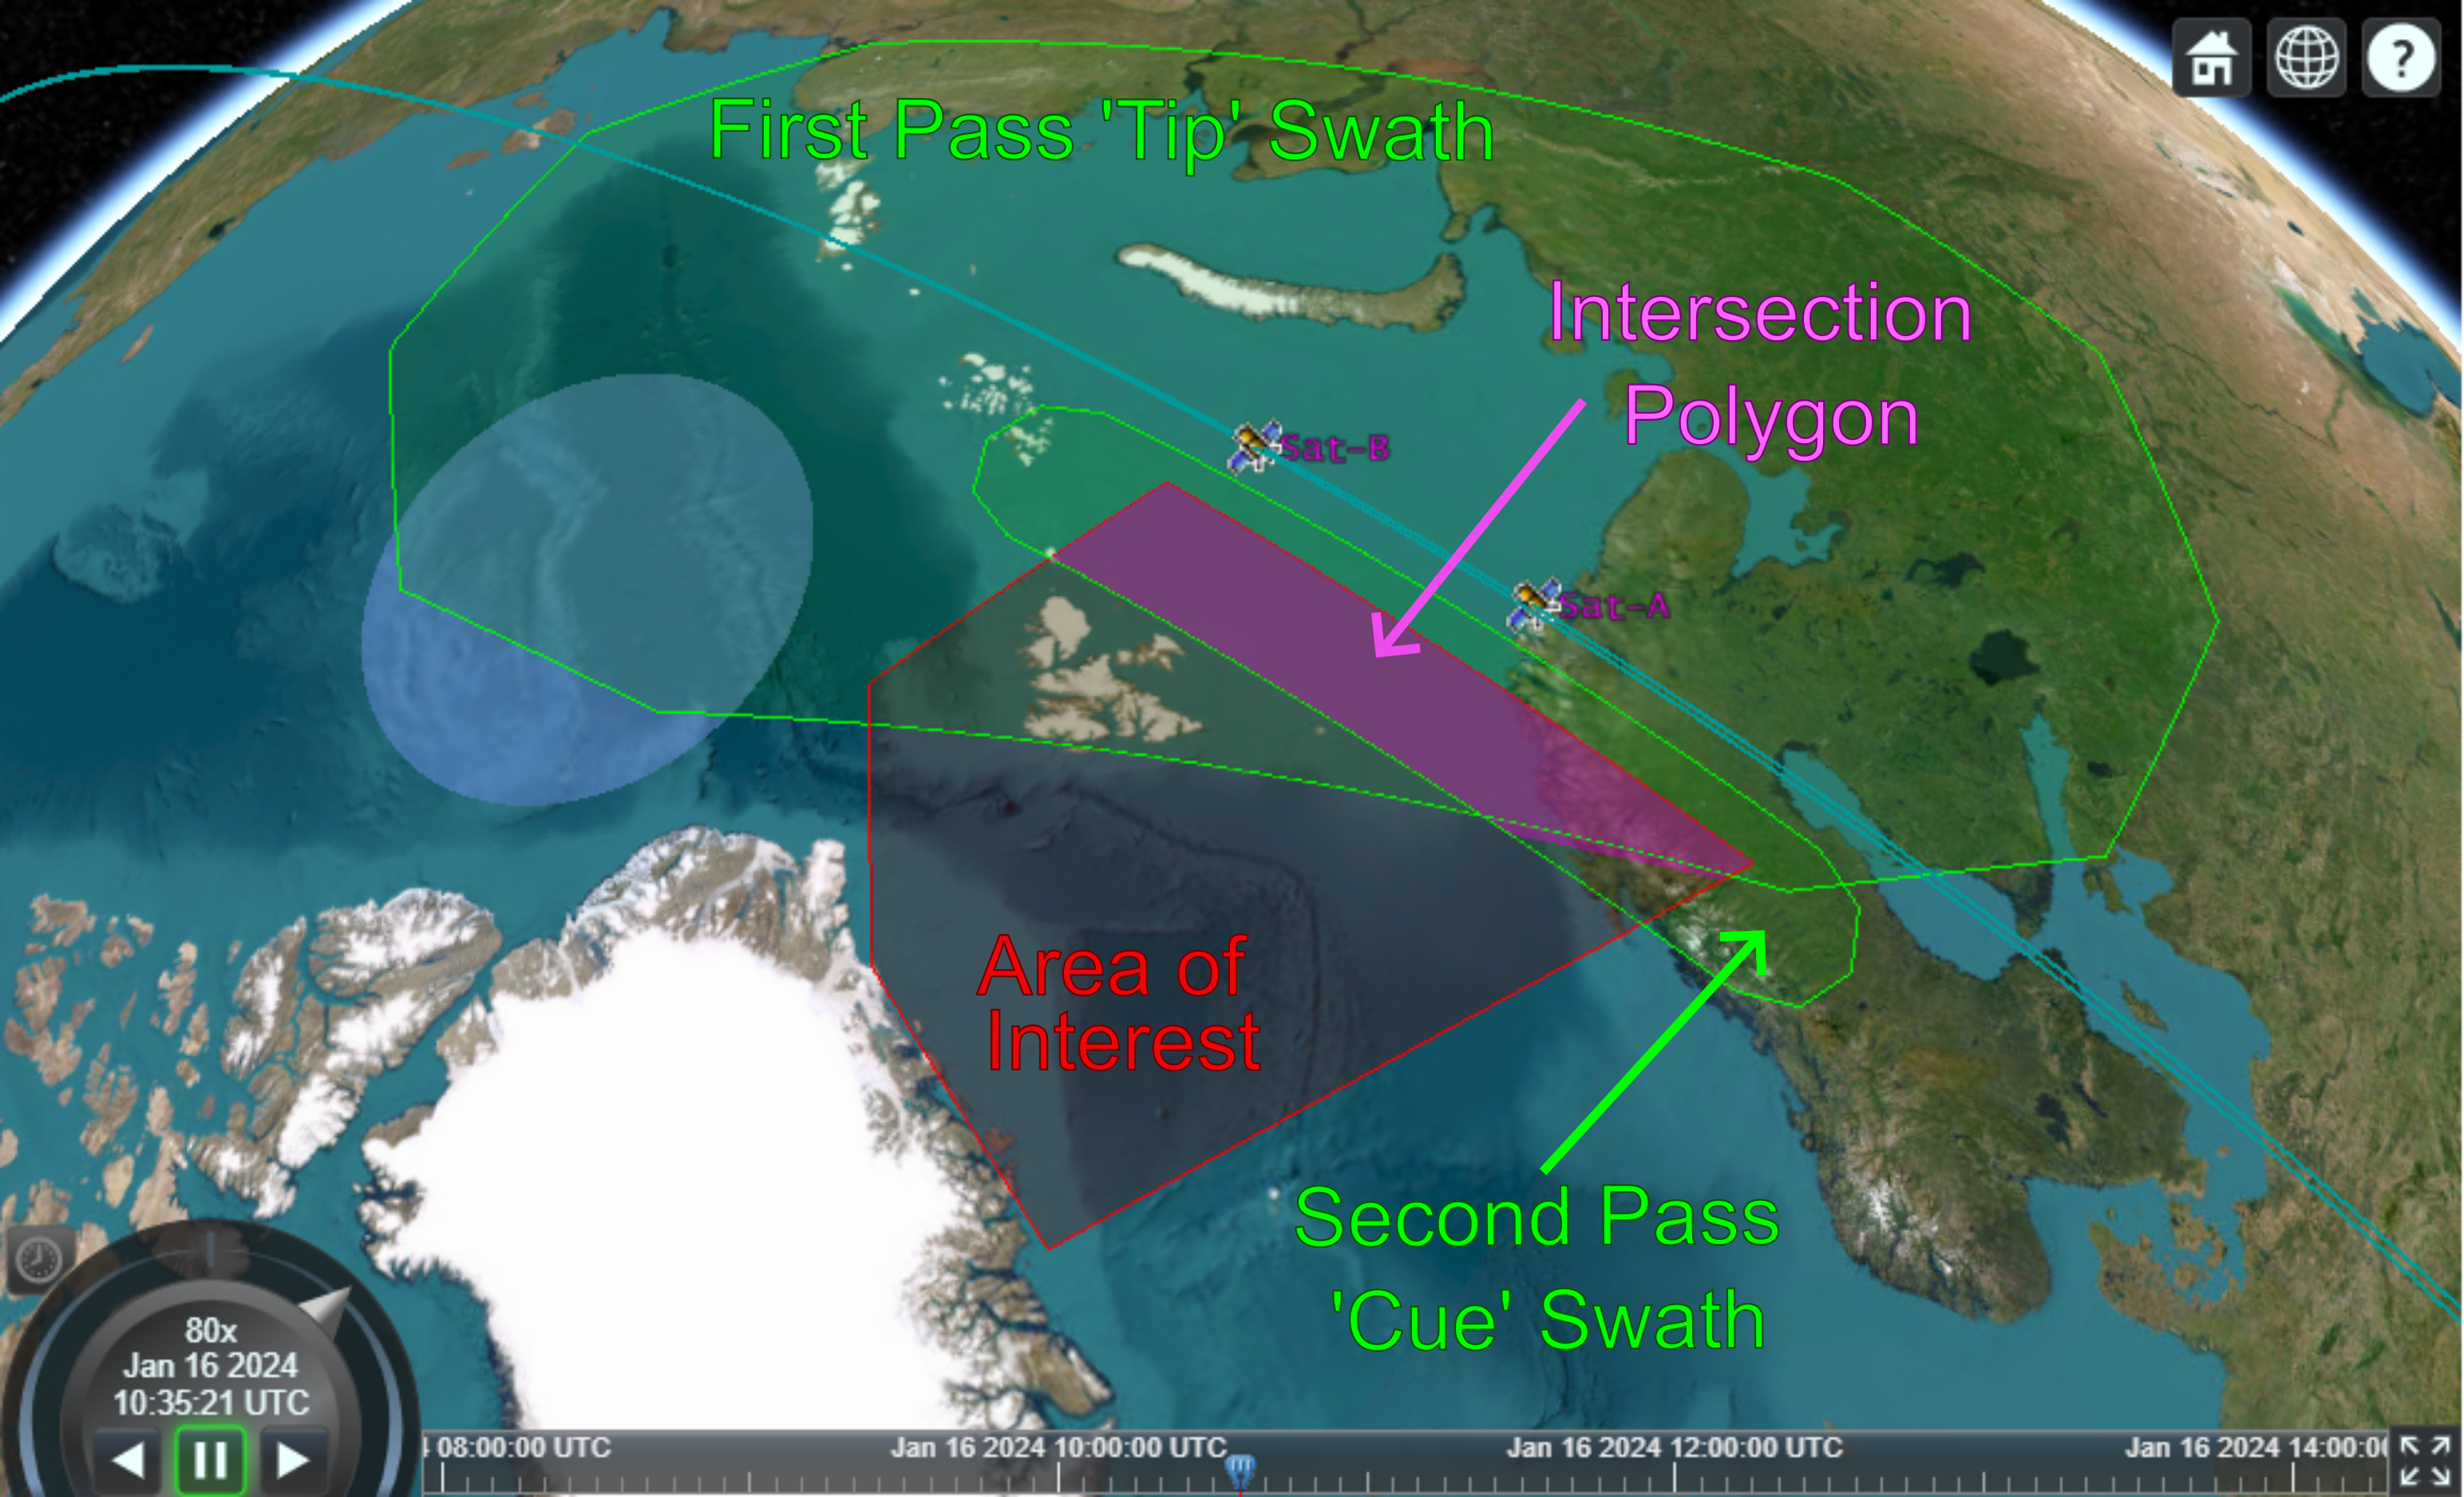
\includegraphics[width=\textwidth]{2023-04-05-POPS-LABELS.PNG} 
%    \caption{Labeled Screenshot of Single Opportunity}
%    \label{fig:screen-2} 
%\end{figure}
%
%\begin{figure}[h] 
%    \centering
%    \includegraphics[width=\textwidth]{2023-04-05-POPS-4.PNG} 
%    \caption{Good Quality Observation Opportunities}
%    \label{fig:screen-3} 
%
%    \includegraphics[width=\textwidth]{2023-04-05-POPS-5.PNG} 
%    \caption{Poor Quality Observation Opportunities}
%    \label{fig:screen-4} 
%\end{figure}


Figure \ref{fig:screen-2}, shows a close-up labeled screenshot of the 3D Earth
viewer.  Here, the \gls{aoi} is represented as a dark polygon with a red
outline, Sat-A and Sat-B’s swaths are visualized in green, and finally, the
intersection polygon is displayed in magenta. For this labeled diagram, the
first-pass ‘Tip’ swath of Sat-A is visualized. This is not done for the
following figures to avoid visual clutter. Also, notice how the intersection
polygon is the intersection area of Sat-A’s swath, Sat-B’s swath, and the
intersection polygon. Part of the purpose of POPS is to enable an operator to
judge the quality of a potential observation. It is clear that the
opportunities in Figure \ref{fig:screen-3} are good quality because they
observe large portions of the \gls{aoi}. The opportunities in Figure
\ref{fig:screen-4} are less desirable because they barely clip the AOI and have
very short access times.


\subsection{Time-Tag Command Generation}

The last stage of the \gls{pops} workflow is \gls{ttc} generation.  At this
point, the operator has created a plan that suits their own needs as well as
their customer’s needs, the plan has been validated, and all that remains is
generating \glspl{ttc} to be uploaded to their specific spacecraft.  Depending
on the observation mode, not all events have commands to be generated. In our
‘EG-SAT’ example case, on the first pass, we may command the satellite to begin
capturing wide-view images. But, on the next pass, we cannot command the
satellite to image potential targets as we cannot know where they will be a
priori. It is known that new commands will be generated between the first and
second pass and, from a planning perspective, this is handled with the
scheduler. The time when these inter-pass commands will be executed will lie
within the second-pass event. In this way, no other \glspl{ttc} should conflict
with the automatically generated commands because if they were scheduled for
that time, they would conflict. 

To generate \glspl{ttc}, templates are combined and populated based on the
observation and the configuration parameters specified when creating the
observation. For example, one parameter may be the duration for which Sat-A
captures images. This value would then be set to an offset parameter in the
templates. 

\begin{figure}[h] 
    \centering
    \includegraphics[width=0.7\textwidth]{timing_diagram.png} 
    \caption{Timing Diagram}
    \label{fig:timing} 
\end{figure}

The generation process is fairly straightforward and specific to each
observation mode on each satellite. But, there are some intricacies worth
noting. Firstly, from the previous example, when creating an observation, the
operator only specifies a duration because that is all they are concerned with.
Generally, for any observation, there are some preliminary and closing
commands. These commands cannot happen instantaneously and may require some
non-negligible margin. It is for this reason that each event is subdivided into
separate timing components. This can be seen in Figure \ref{fig:timing}. The
start and stop times are the same as the event’s start and stop but they
specify when the first \gls{ttc} is executed and when the final \gls{ttc} has
concluded its execution respectively. The epoch is the time when the
observation begins sensing and the duration is the period after which the
sensing is performed. As part of the \gls{ttc} generation capabilities, these
timings can be determined programmatically by evaluating the templates for each
observation. As such, when an observation is created by the operator in the
observation configuration stage, they specify the epoch and the duration, and
the \gls{ttc} generator determines the start and stop times.






\glsresetall{} 

%\chapter{Discussion and Future Work}\label{chap:discussion}
\chapter{Future Work}\label{chap:discussion}

%\lettrine[lines=2, findent=0pt, nindent=5pt]{A}{} 

At the time of writing this thesis, the \gls{pops} is still very much in
development. The project began in 2021 and has undergone continuous work since
then. In the following sections some some areas where \gls{pops} needs to be
developed and improved are discussed. Some of these are critical updates that
are necessary for the \gls{mvp} and others are important for the general health
and functionality of the tool.

%When designing something
%that is completely unique and as ambitious as a mission planning tool, it is
%difficult to gauge the work required to meet its requirements. Before,
%discussing future directions for the tool, it would be helpful to first go
%over how \gls{pops} became what it is. 

%\section{Research and the Development Process}

%Early on in development, much effort was put into exploring possible tools,
%languages, and frameworks to build from. Initially, before the creation of the
%Propagator service, the intention was to rely on an open-source tool,
%developed by NASA, called the \gls{gmat}. \gls{gmat} is well made and designed
%to model, optimize, and estimate spacecraft trajectories
%\cite{hughes_using_2017}.  Originally, it was thought that it could act as a
%replacement for the \gls{stk}. It could be used to take \glspl{tle} and
%generate ephemerides.  \gls{gmat} comes with its own propagators and the
%software could be run from the command line. Given a script representation of
%a mission, ephemeris data could be generated in the form of a report.
%Unfortunately, SGP4 was not supported by the software (though this was added
%in a 2022 release) which made \glspl{tle} unusable given this approach.
%\gls{gmat} could be expanded as it has a very well designed plugin interface.
%Theoretically, an open-source implementation of an SGP4 propagator could have
%been implemented into \gls{gmat}.  Then the question arose, if a propagator
%needed to be added, what was \gls{gmat} providing?  Upon evaluating this
%approach, it was determined that using \gls{gmat} in this way added a great
%deal of work. As well, some issues were: \gls{gmat} was restricted to a
%windows environment, data needed to be transferred through a \gls{tcp}
%connection, and generating mission scripts was convoluted. This is not to say
%that this time was wasted; rather, this was time spent exploring a useful tool
%that ended up being inadequate for \gls{sfl}'s purposes. 

%% Mention in the prop section that GMAT was originally used and then replaced by an open source library


%https://gmat.atlassian.net/wiki/spaces/GW/overview
%https://core.ac.uk/download/pdf/80605179.pdf

%Similar work was done for another NASA tool called, OpenSPIFe. Its purpose was
%to handle scheduling and planning. Very similar to \gls{gmat}, it provided a
%great deal of functionality that could be updated and developed. Similarly,
%this tool would have increased the amount of work for any developer working on
%the project. For any tool that is used, developers must take responsibility
%for it to at least understand how to use the tool but also make changes if
%bugs appear. For both \gls{gmat} and OpenSPIFe, it was determined that the
%overhead for developing the tools from scratch would be far less than having
%to maintain two tools, which are fully fledged projects in their own rights
%developed by teams of professional software engineers.

%Since the decision was made to move to develop a mission planning tool from
%scratch, development became more productive than exploratory. The first
%service developed was the Propagator service. Ephemeris data is fundamental to
%every aspect of \gls{pops} so it was essential. Here was a situation where an
%open-source library was more helpful than it was burdensome. Well tested
%implementations in many languages of the SGP4 algorithm are made available
%along with \cite{vallado_revisiting_2006}. These implementations, though, are
%only of the algorithm itself and not any surrounding functionality such as
%coordinate frame transforms or generating an ephemeris. This is where a
%separate open-source Python implementation of SGP4 code was found. It was
%based on the same source code from \cite{vallado_revisiting_2006} and it
%provided a library of helper functions that enabled all of the surrounding
%functionality.  This allowed efforts to be focused on validation and on using
%the ephemeris data rather than generating it.

%It is of the utmost importance that a developer conforms with the license
%associated with a library so as to not be exposed to litigation. Most
%important is whether a library requires that the source code of the software
%that makes use of library must be disclosed to the public. A `copyleft'
%license requires that derivative works must disclose their source code. The
%\gls{gpl} license is a very common copyleft license.  Conversely, a
%`permissive' license makes no obligations to derivative works. The \gls{mit}
%license and Apache License are very common examples of permissive licenses.
%With this in mind, time was spent ensuring that all of the open source tools
%used by \gls{pops} fell under the permissive category. 

%% Mention licensing in the intro potentially

%This was especially a challenge for Cesium as . Other libraries existed that
%supported a 3D Earth visualization. These were basic and would require a great
%deal of work to become usable. Cesium provided the most functionality with the
%best \gls{api}. As such, it was worth investing time in.  Recall that CesiumJS
%is the open source library that most of the functionality of the tool is built
%on.  CesiumION is the proprietary version and provides 3D geospatial data
%which includes world maps, terrain data, and specialized objects within the
%viewer.  For the world map, as long as it is cartographically accurate, it is
%sufficient for \gls{sfl}'s purposes. For example, as part of \gls{pops} there
%is no need for high resolution imagery of downtown Toronto.  Similarly, there
%is no need for terrain data for a space application.  Time was spent looking
%for free alternatives, which were found.  As such, there was no reason to pay
%for a license to CesiumION when free alternatives existed.



%After Cesium was made usable, most of the tools were in place to begin full
%development of \gls{pops}. This began with foundational work setting up a
%basic website that could be interacted with. Initially, it was very simple and
%had a number of menus that could be used to create missions, add satellites,
%add ground stations, and configure a plan. From this began work on the
%observation configuration page which was the most complicated aspect of
%\gls{pops} yet developed. It needed to interact with all the tools that had
%been introduced.  Not only that but it also needed to search for
%opportunities.

%Opportunity searching was the most difficult aspect of \gls{pops}. It is
%completely unique, in that there existed no open-source tool that could be
%configured to find remote sensing opportunities given some constraints. Of
%course, \gls{stk} could be used, but it would require a license and would need
%to be automated in some way. Other tools like \gls{cpaw} could be used but
%again they provided superfluous functionality and require licenses. This
%process would need to be done from scratch. Before beginning development, a
%document was written that fully defined all of the initial observation modes
%that were desired as part of \gls{pops}. Information like: what satellites
%were necessary for a particular observation; can one, some, or all be used;
%explicitly defining what constraints were necessary; defining what terminology
%was being used; etc. This document was then reviewed to ensure that there was
%a correct understanding of what was required.

%Originally, just the \gls{atu} were thought to be sufficient for opportunity
%filtering. Through the creation of this reference document, it became clear
%that in isolation, the \glspl{atu} could not fully constrain the observation
%modes as described in the document. Strung together, they could do so.  This
%is how the flow-charts similar to Figures~\ref{fig:filter-1} and
%\ref{fig:filter-2} from Chapter~\ref{chap:intro} were created. They
%summarized, at high level, how the \glspl{atu} could be used to fully
%constrain an observation. They were easy to understand and adaptable. It
%followed that the implementation of the opportunity filter should be as simple
%as these high level diagrams. In response, the filter was split into a number
%of classes that emulated the flow-diagrams. The Data Handler classes
%represented the data at varying stages, such as: the Ephemeris, \gls{aoi},
%Swaths, Polygons, and Access Times. The \gls{atu} Handler, could use the data
%handler classes as inputs and outputs. Finally, the Opportunity Filter class
%would use the other two classes to fully implement a filter.  

%% Add a point in the intro that the ATUs were thought to be sufficient
%% Also mention how the different classes are used to replicate opportunity filtering

%Implementing these filters required iteration. Not just for efficiency but
%also because each version made assumptions about the filters that artificially
%limited the filter's capabilities.  It is very difficult to plan and account
%for each aspect of the filters before-hand.  For example, the temporal
%properties of the Tip-and-Cue Imaging observation had some hidden challenges.
%From a high level, it is very simple: (1) first pass tip access, (2) ground
%contact, and (3) next pass cue access. The initial solution may be to iterate
%through each pass for a scenario. For each pass, the access time between Sat-A
%and the \gls{aoi} are found. Then an access between Sat-B and the intersection
%polygon from the Sat-A \gls{aoi} access is calculated. If that access exists
%and if there is a ground contact, all the information is stored as an
%opportunity.  This is essentially what is currently being done as outlined in
%Algorithm~\ref{alg:tip-and-cue} in Chapter~\ref{chap:architecture}.  
%
%This solution is technically valid, but what if there are multiple Sat-A
%\gls{aoi} accesses in a single pass? Or, what if there are multiple Sat-B
%intersection polygon accesses? Then, this process of iterating over passes may
%miss potential opportunities. The solution needs to be improved and instead of
%looping over every pass, the filter should iterate over every Sat-A \gls{aoi}
%access.  In this way, a tip opportunity is never missed. Then, the filter
%should intersect the tip intersection polygon with the first Sat-B intersection
%polygon on the next pass.  This is just one example of how the process needs to
%be iterated.  Other sources were effectively managing the data in a scenario.
%Specifically how should data be stored such that it can be used as needed
%throughout the filtering process, how to prevent copying the data
%unnecessarily, or how to provide data to the \glspl{atu} effectively such that
%the filter wasn't slowed down unnecessarily by performing repeated or
%superfluous calculations.  

%% Maybe move the last two paragraphs to the architecture section

%The last area that slows down development is bug fixing and stability
%improvements. This nothing special; any part of a development workflow will
%require ironing out bugs. Given the scale of the tool, part of the attitude
%when developing has been making things perfect takes a lot of time so make it
%good enough to work for now. This is perfectly valid, and makes sense.  There
%is neither the time nor the resources to support optimizing every aspect of
%the tool. That being said, expanding the tool requires building on itself.
%Much of the functionality is inter-reliant and very little can be done in
%isolation. If we fully followed a ``get it done'' mentality, the tool would
%quickly fall in on itself. For this reason, a great deal of time has been
%spent iterating on every aspect of the tool to make it more robust, such that
%when new functionality is added, it is not limited artificially or it does not
%cause the tool to collapse in on itself.

%\section{Future Work}

%With some understanding for how \gls{pops} was created, some areas where
%\gls{pops} needs to be developed and improved can be discussed. Some of these
%are critical updates that are necessary for the \gls{mvp} and others are
%important for the general health and functionality of the tool.

\section{Time Tag Command Generation}

The most critical aspect of \gls{pops} that must be developed is the \gls{ttc}
generation functionality. It is an essential component of the tool and cannot
be omitted. There are two aspects to this. First, the functionality for
generating \glspl{ttc} must be developed and, second, the necessary \glspl{ttc}
for each observation mode must be determined.

Work has been done to implement \gls{ttc} generation. There exists a library
developed by \gls{sfl}, written in Python, that handles the logic for creating
\gls{nsp} commands. Work was done to re-tool this library to generate
\glspl{ttc} from these \gls{nsp} commands. A service was created around the
re-tooled library to generate list of \glspl{ttc} for each observation mode.
The intention for this service was to be expandable and easy to use for future
developers since \glspl{ttc} used for each observation mode will change from
mission to mission. This is where the intricacies discussed in
Section~\ref{sec:ttc-gen} where discovered.  

For a number of reasons this approach was not used. The \gls{nsp} library did
not explicitly track the data payloads of the \gls{nsp} commands.  That is, the
library could construct valid commands but they did not track mission-specific
information.  For example, if a command were to be sent to the \gls{hkc} on the
satellite, the developer would have to write the address itself within the
code. This makes development more difficult since a developer would need to
have knowledge of the commands themselves, rather than having that
functionality be handled by the software.  Typically, for ground software at
\gls{sfl} this is handled by \gls{xml} configuration files that are configured
for each new mission.  The \gls{nsp} library did not make use of these
configuration files because it was designed for testing purposes and not
necessarily for use in nominal operations. So, when using the Python \gls{nsp}
library, individual data bits would need to be specified in Hexadecimal. In
addition, it was decided that using Python scripting to generate \glspl{ttc}
may be too cumbersome for future developers. Because of these issues, the
service was replaced by a new tool that builds off \gls{xml} configuration
files as the foundation for \gls{ttc} generation.  This tool is still in
development.  

Determining what commands are necessary for each observation mode can be
challenging.  Necessary commands may be: powering on devices in the spacecraft,
setting profiles, arming and disarming these profiles, specifying where in
memory where data should be stored, specifying the necessary duration for
commands, specifying attitude modes, etc.  There does not exist a single
reference for what commands are necessary and what must be done for an
observation mode. This information can only be gained through discussion with
operators and with software engineers developing the firmware.  Even after
extensive consultation, there is potential for steps being missed. It is only
through testing, are all of the necessary commands for an observation mode
determined.  Thankfully, much of this testing can be done during \gls{tvac}
testing campaigns. It is here, were spacecraft may be commanded to perform
observations, or at least their ground analogues, through \glspl{ttc}.  This
gives a great deal of information about what specifically needs to be performed
for each observation. It also provides some means of validating \gls{ttc}
generation.


\section{Validation}

The next most important aspect of \gls{pops} that must be accomplished before
an \gls{mvp} is ready, is validation. The tool must yield acceptable and
accurate results. System level validation can be accomplished through
service-level verification. This has been touched on throughout the thesis.
Specifically, the Propagator service was validated through comparing ephemeris
data with results from \gls{stk}. \gls{ttc} generation validation may be
accomplished through \gls{tvac} testing. After this, the \glspl{atu} may be
individually validated either through known test cases or through comparisons
with \gls{stk}. This process has been handled separately.  For opportunity
filtering, there does not readily exist an alternative that can act a
benchmark. In the future, what may be done is when the filtering process has
reached maturity, simple test scenarios will be constructed for each
observation mode.  \gls{stk} and \gls{pops} will separately be used to search
for opportunities and these results will be compared. Currently, there is not a
requirement for some of the components. Developing validation strategies is an
ongoing process.

%For example, a high accuracy with respect to access times is not necessary.
%Even if the access time calculation were made very accurate, there are
%inherent uncertainties in the ephemeris data that may render such accuracy
%useless.
 
%\subsection{Addition of More Observation Modes}
%
%Some missions that \gls{pops} is intended to be used for require additional
%operations modes beyond just what was discussed in the 

\section{Performance}

Currently \gls{pops} has issues with large amounts of data. For scenarios
longer than a few days, storing and retrieving data, displaying information,
and opportunity filtering becomes slow. To illustrate this, let us run a simple
benchmark test. For this test, we will run the Tip-and-Cue Imaging opportunity
filter for a number of scenarios, each with an increasing scenario size and a
10s timestep. Each scenario will have two satellites (Sat-A and Sat-B), three
ground stations (\acrshort{sfl}, ESCS, and GSW), and the same \gls{aoi}
discussed in Chapter~\ref{chap:workflow}. The reason we'll use the opportunity
filter as a benchmark is that it interacts with almost every part of \gls{pops}
and Tip-and-Cue Imaging is the more complicated observation mode.
The purpose of this test is not to give an in-depth characterization of the
performance of \gls{pops} but rather its purpose is to give a rough idea of its
potential.  These scenarios were run on a laptop with 40GB of RAM and an
$11^{th}$ generation Intel Core i7-1165G7 CPU running at 2.80 GHz. 


\begin{figure}[h]
    \centering
    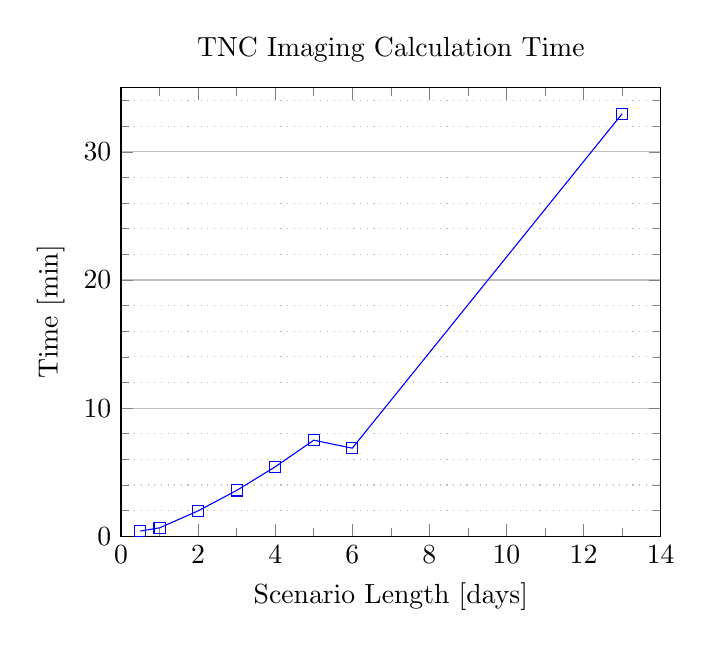
\begin{tikzpicture}
    \begin{axis}[
	title={TNC Imaging Calculation Time},
	xlabel={Scenario Length [days]},
	ylabel={Time [min]},
	xmin=0, xmax=14,
	ymin=0, ymax=35,
	xtick={0, 2, 4, 6, 8, 10, 12, 14},
	minor x tick num=1,
	minor y tick num=4,
	ymajorgrids=true,
	yminorgrids=true,
	minor grid style=dotted,
    ]

    \addplot[
	color=blue,
	mark=square,
	]
	coordinates {
	(0.5, 0.400643333) (1, 0.651415) (2, 1.976971667) (3, 3.57072) (4, 5.415478333) (5, 7.492456667) (6, 6.871896667) (13, 32.980525)
	};
	
    \end{axis}
    \end{tikzpicture}
    \caption{Simple Opportunity Filtering performance benchmark}
    \label{fig:performance-benchmark}
\end{figure}

The results of this test can be seen in Figure~\ref{fig:performance-benchmark}.
As can be seen from the plot, 8 scenarios were generated. Scenarios less than 4
days are reasonably quick, taking less than $\sim5$ minutes. But, as we
approach a 13-14 day scenario filtering takes more than half an hour. It could
be argued that this is tolerable for an \gls{mvp} but it is certainly not
ideal.  Note, this test was only for a 2-satellite scenario. Every satellite
added increases the running time exponentially. 

To address this, there are a number of areas for improvement to consider.
These range from simple algorithmic changes to heavily involved architectural
changes. For each change, work will need to be done characterizing what is
taking up the most time to justify the change. Some possible avenues for
improvement, in increasing difficulty, are:

\begin{enumerate}
    \item Making ephemeris data dynamic,
    \item Splitting up the data in the filtering process,
    \item Utilizing parallel computation,
    \item Offloading computation to a dedicated server, or
    \item Leveraging the GPU
\end{enumerate}


\subsection{Making Ephemeris data dynamic}

Ephemerides are generated for each satellite once when a plan is created. This
ephemeris data has a set time range and timestep. It is here a user must decide
whether they want an accurate but slow to process plan, or an inaccurate but
fast plan. Why should they be required to make this decision? Or, at least, why
should this decision be made once and then be set in stone for the duration of
the plan? What's more, if the timestep is constant for an entire plan, it is
likely that, for small timesteps, most of that data is wasted. If a user is
concerned with an \gls{aoi} in the Northern Hemisphere, they will not need a
high accuracy ephemeris for times where the spacecraft is in the southern
hemisphere. Of course, if the user is concerned with a very large \gls{aoi}
that the spacecraft more often than not has access to, then nothing can be
done. This, though, is an outlier case.

This touches on potential improvements for how ephemerides can be better
handled.  Instead of initially making a large ephemeris with a small timestep,
a rougher, large timestep, ephemeris could be generated.  For periods where
high accuracy is needed, such as when there is an access, ephemeris data could
be dynamically generated in that area specifically to increase the accuracy
where it is needed. Or, conversely, a small timestep ephemeris could be
initially generated, then after the calculations are performed, unnecessary
data could be omitted. These are both general ideas for now and would need
dedicated development time to plan out and troubleshoot any pitfalls.

In terms of difficulty, this would require a re-work of a large portion of
\gls{pops}.  Thankfully, through abstracting how ephemeris data is handled
through the Data Handler classes, \gls{pops} is well situated for this change.
Overall, this is a change that will likely be made later.  Having ephemeris
data be static artificially limits \gls{pops}'s functionality.


\subsection{Splitting up data in the filtering process}

Currently, during opportunity filtering, all of the data is loaded for the
entire scenario. That being ephemeris data, swaths, access times, etc. If
having all of this data loaded in at once is causing the filtering process to
slow down, it may be better to instead load the data in chunks. For example,
for a 14 day scenario, instead of loading in all 14 days of data, this could be
split up into 2 day chunks. This will likely not reduce the processing time but
it may reduce the time spent indexing and accessing the data. In terms of
difficulty, this would be an easy modification but time would need to be spent
determining whether this change is worthwhile.


\subsection{Utilizing parallel computation}

Moving from single-threaded processing to multi-threaded processing begins to
stray from algorithmic changes to a change in how the host PC is utilized.
These solutions, while most likely effective, increase the complexity of
\gls{pops} and should be pursued if there are no other alternatives.

Thankfully, opportunity filtering is well suited for multi-threaded
programming. Searching for opportunities is done through brute-force numerical
computation, and many of the calculations are performed independently from each
other. A system could be developed that splits the filtering process into a
number of processes, each handling sub-components of the filtering process. 

This would be a difficult solution to implement. Multi-threaded programming is
not necessarily complicated in Python, but asynchronous processes are almost
always much more complicated than asynchronous process. Synchronous processes
are predictable, straightforward, and easy to debug. Asynchronous processes are
none of these and introduce a multitude of challenges. For example: race
conditions, memory management, locking out resources, unpredictable behavior,
error handling, etc.  There are many benefits to parallel computing, but such a
change should not be undertaken lightly.


\subsection{Offloading computation to a dedicated server}

When performing opportunity filtering, or any other function of \gls{pops}, if
other software is being run on a user's computer, that may negatively impact
the tool's performance. Or, if the user's computer is not particularly
powerful, that may limit \gls{pops}'s usefulness. Instead, a dedicated server
could be constructed that is optimized to perform calculations for \gls{pops}.
Some calculations may be: ephemeris generation, the \glspl{atu}, database
management, and opportunity filtering. In this way, all that a user's computer
will run is what they need to display the information or construct requests.
Alternatively, all of \gls{pops} could be hosted on a server, and a user could
access it completely remotely. 

There are potential benefits to this approach, but it would vastly increase the
complexity of \gls{pops}, especially for the front-end user interface. Some
difficulties would include: managing data transfer, tracking user sessions, or
potentially removing functionality from the Mission Model service. The issue of
tracking user sessions is particularly difficult. If a user runs \gls{pops} on
their own computer, it can be assumed that only they will be interacting with
the webserver. But, if the server is hosted remotely, then the webserver needs
to track both what requests are being sent to it as well as from what source.
For example, let us say there are two users who wish to work with two different
plans. User 1 will open Plan A and the webserver will display Plan A. User 2
will open Plan B and Plan B will be displayed. Suppose then User 1 makes a
change to Plan A, the webserver will receive the request but, since it isn't
tracking from what source are the requests coming from, it will make changes to
Plan B since that was the last plan displayed.  The behavior is undefined and
both User 1 and User 2 will have unstable sessions.  In this way, sessions
should be split somehow, such that one user's inputs cannot affect another
user. This problem has many solutions but is non-trivial and strays into
professional web development which is not the priority for \gls{pops}. 


\subsection{Leveraging the GPU}

So far, all computation has been done on the \gls{cpu} which is general purpose
but slow. The \gls{gpu} is optimized for computer graphics and image
processing. Specifically, they are built to process large blocks of data in
parallel. They are especially good at handling any process that uses linear
algebra. Historically, \glspl{gpu} were only meant to be used for computer
graphics but recently, they have become much more general purpose. By
leveraging the \gls{gpu}, computation times may be decreased by orders of
magnitude. Some precedent does exist for this by accelerating SGP4 calculation
\cite{moeckel_high_2016} \cite{fraire_opencl-accelerated_2013} and it is
reasonable to assume this can be expanded further.

Using a \gls{gpu} would be the most rewarding but also most difficult and
complicated improvement to \gls{pops} that could be made. Writing code for a
\gls{gpu} is to some extent specific to the manufacturer and age of the
\gls{gpu}. Some computers that may run \gls{pops} may not even have a \gls{gpu}
that supports this functionality. So in addition to creating the custom shaders
for \gls{pops}, work would need to be done to ensure that they can be used by
users at \gls{sfl}.
 

\subsection{Miscellaneous Improvements}

In addition to any large improvements, there exists many smaller changes that
can have a positive effect on \gls{pops}'s performance. Small changes such as:
dynamically loading data from the database, sending multiple batches of data to
the \glspl{atu} in a single HTTP request rather than multiple HTTP requests, or
optimizing data formats based on need.


\section{Updating Plans}

Another area that must be improved is the ability to update plans in
\gls{pops}. Currently, once \glspl{tle} are set for a plan, they cannot be
changed. This was done to reduce the complexity of the tool but this is not an
ideal solution.  Suppose a plan has been made and observations have been
scheduled, but then suppose after some time a new \gls{tle} is generated that
invalidates the observations made with the older \gls{tle}. This is a
reasonable scenario that could very well occur but currently there is no way to
handle this in \gls{pops} aside from creating a new plan and rescheduling
observations.

This is a multi-faceted problem that must be addressed in a number of areas.
First, it must at least be determined if a new \gls{tle} invalidates
observations from a plan with a previous \gls{tle}. Next, there must be a way
to edit observations in an old plan or there must be a way to migrate those old
observations to a new plan with updated timings. Lastly, if a change is made to
an observation, \glspl{ttc} that have already been generated must be updated in
some way to reflect those changes. This problem has not yet been approached and
is an on-going limitation of the tool.


\section{Communication With Other Ground Software}

\gls{pops} is not meant to be used in isolation. It is important that it is
able to communicate with other ground software at \gls{sfl}. Specifically,
\gls{pops} must be able to read commands that are scheduled for different
spacecraft. This is necessary for planning and scheduling.  Without an
understanding of what is already planned for a satellite, observations that a
user adds may conflict with existing \glspl{ttc}.  How exactly \gls{pops} will
interact with \gls{sfl}'s ground software has yet to be determined.  

This additional functionality is planned to be an additional class which acts
as an interface between the scheduler class and \gls{sfl}'s ground software. It
is here uploaded \glspl{ttc} will be read and added onto the schedule.



\section{Testing}

The last task that must be performed before \gls{pops} has reached the
\gls{mvp} is user testing. Quite simply, this is where operators begin to use
the tool and give feedback. This information is critical since it gives insight
into: bugs, user interface problems, and what parts of the tool can be
improved.  This then begins the process of iterating in their feedback,
improving the tool, receiving further feedback and so on.


         
\glsresetall{} 

\chapter{Conclusion}\label{chap:conclusion}

\lettrine[lines=2, findent=0pt, nindent=5pt]{T}{} his thesis has discussed
the purpose, design, and implementation of the \gls{pops} developed by the
\gls{sfl}. \gls{pops} is being developed to address the need for mission
planning capabilities for the operations at \gls{sfl}. It is not intended to
fully automate an operator's workflow but rather its purpose is to streamline
some of their day to day activities. The main design direction for this tool
has been to keep it easy use and easy to develop. Many tools have been
developed at \gls{sfl} that have fallen into obscurity. Even if the tool is
very efficient, this is less valuable than a tool that can be expanded into the
future. 

Existing software solutions to mission planning that are currently available
have been introduced. Their strengths as well as their weeknesses have been
discussed. After this some terminology was introduced as well as some
operations related concepts. Since it is not the desire of the author to expose
the operations strategies of \gls{sfl} customers, an example scenario was
defined, EG-SAT, to illustrate the usefullness of \gls{pops}.

After this, the architecture of \gls{pops} was discussed. Starting with the
general architecture of the software. Then going into the specifics of each
service, those being the: Propagator, Database, Access Time Utilities, NSP
service, and Mission Model. Each has its own purpose and the largest is the
Mission Model. It handles the front-end user interface, communication with the
database, opportunity filtering, data handling, and event scheduling.

Just discussing the architecture does not fully explain the purpose of
\gls{pops}. To help aid in this process, a workflow was discussed for the
EG-SAT mission. Starting with setting up \gls{pops} for a mission, adding
satellites, and ground stations. After this, a plan was set up for a 3-day
period. There, opportunities were searched for given EG-SAT's two operations
modes, Coarse Imaging and Tip-and-Cue Imaging. From these opportunities,
observations were created and added to the schedule. The schedule was then
validated and displayed.  

A great deal of work lies ahead for \gls{pops} but this is only a testament to
the amount of work that has already been accomplished. Hopefully, this tool
will at least provide some benefit to operators at \gls{sfl} for many years to
come.










           
\glsresetall{} 
\appendix

\chapter{Algorithms} \label{chap:Algorithms}

\lettrine[lines=2, findent=0pt, nindent=5pt]{T}{} hrough the development of the
\gls{pops}, a number of algorithms have been developed to perform various
functions. These algorithms are not necessarily ground breaking but their
implementations are novel and worth discussing in some form. To avoid
detracting from the main body of the thesis they have been placed here, in the
appendices.


\section{Multiple Access Intersection Algorithm} \label{alg:mul-access-inter}

For some search scenarios, we may need to determine for what times do all
satellites have access to a target such as an \gls{aoi} or a ground station.
That is, if we have more than one satellite and each satellite has a list of
access times to a target, we must generate a new list of access times where
each access corresponds to a period where all satellites have access. An
example scenario is illustrated in Figure \ref{fig:access_intersect}.


\begin{figure}[h]
    \includegraphics[width=\textwidth]{Access Intersection Example.png} 
    \caption{Illustration of a Potential Access Intersection Scenario}
\label{fig:access_intersect}
\end{figure}

In this scenario, there are three satellites: Sat 0, Sat 1, and Sat 2. Each has
multiple access periods represented with gray boxes. Though time is continuous,
it has been discretized into integer timesteps for simplicity. Minutes have
been selected as the units for time but this is arbitrary. From these lists of
access periods, this algorithm must determine all of the points in time where
all satellites have an access period. For the example scenario, the outputted
results should be $[7,10]$ and $[28,36]$. Note that between $t = 16$ and $t=22$
there are access overlaps but since there are only overlaps between two
satellites, they should not be returned as intersection periods.

For a satellite, access times are stored as a list of timestamps. Every even
and odd indexed timestamp specifies when the satellite `enters' and `leaves' an
access respectively. Access lists $\ses{a}{n}$ can be described generally for satellite $n$ as,

\begin{equation} 
    \ses{a}{n} = \left[ a_{n,0}, b_{n,0}, a_{n,1}, b_{n,1}, \ldots a_{n,m}, b_{n,m} \right]
\end{equation}


where $a$ is the access enter timestamp, $b$ is the access leave timestamp, and
$m$ is the number of accesses. We also make the assumption that no accesses
overlap for a given satellite and target; that is,

\[
    a_{n,0} < b_{n,0} < a_{n,1} < b_{n,1} < \ldots < a_{n,m} < b_{n,m}
\]

One simple brute force solution to this problem would be to iterate over every
time step, $t$, and check if there exists an access region, $[a_n,b_n]$, for all
satellites, $n$, such that $t$ is between $a$ and $b$.

This solution is, of course, very wasteful as it scales with the number of
timesteps that are being considered, $\Theta(t)$. The number of timesteps may
be on the order of 1,000s to 10,000s of timesteps. A simplification can be made
since we do not need to actually consider every timestep. Rather, we can
instead iterate over the access boundaries since they describe continuous
periods of time. By focusing on just the access boundaries, we may develop an
algorithm which scales with the number of accesses, $\Theta(m)$, which is much
smaller than the total number of timesteps.

For all satellite access lists we are considering, let us combine them into two
$1\times nm$ arrays. The first `timestamp' array, $\se{b}$, contains a sorted
list of all of the boundary timestamps in ascending order. The second `index'
array, $\se{s}$, contains a list of satellite indices in the same order as the
timestamp array. For example,

\begin{equation*}
    \begin{aligned} 
	\ses{a}{0} &= \left[ 2, 10, 18, 21  \right] \\
	\ses{a}{1} &= \left[ 4, 12, 16, 19  \right] \\
	\ses{a}{2} &= \left[ 7, 15, 20, 22  \right] \\
    \end{aligned}
    \quad \Rightarrow \quad
    \left \{ 
	\begin{aligned}
	    \se{b} &= [ 2 , 4 , 7 , 10 , 12 , 15 , 16 , 18 , 19 , 20 , 21 , 22  ] \\
	    \se{s} &= [ 0 , 1 , 2 , 0 , 1 , 2 , 1 , 0 , 1 , 2 , 0 , 2  ]
	\end{aligned}
    \right.
\end{equation*}

Note these are some of the values from Figure \ref{fig:access_intersect}.
Again, in the actual implementation of the algorithm we use actual timestamps
but here we are using integers for demonstration purposes. The timestamp array
stores the timestamp of the access boundary for later reference and also gives
us the order of the satellite index array. Now with the index array we can do
something interesting. Remember that access boundaries are listed in order of
[enter, leave, enter, leave, etc.]. Looking at the first four elements in the
index array, $[0, 1, 2, 0]$, satellite 0 enters an access at the first element
and leaves the access at the fourth element. So for the second and third
element, satellite 0 still has access because it has not left yet. In essence,
the index array encodes in what order satellites enter and leave accesses. 

Now let us expand on the index array so we can perform logical operations to
find intersections. For this the algorithm makes use of logic arrays.  These
are arrays which contain only boolean values, True or False. With these arrays,
we can also perform logical operations on any axis. For example, if we have a 2
dimensional logic array, we can produce a 1 dimensional array, that is the
result of AND'ing all of the elements in each column. These allow us to perform
logical operations very quickly for many elements. From the index array let us
construct an $n\times nm$ boolean array, $\se{A}$, that describes our scenario.
The rows of matrix, $\se{A}$, correspond to the indices of each satellite.  For
example row 0 is satellite 0, row $m$ is satellite $m$, etc. The columns
correspond to elements in the index array, $\se{s}$.

Let us initialize $\se{A}$ to be all False values represented as 0s. Then,
starting at the first column of $\se{A}$, let us NOT the element in the
$\se{s}(0)$ row.  Then, for then next column, let us copy all of the values
from the previous column and again NOT the $\se{s}(1)$ element. This is then
repeated for all columns in $\se{A}$. There is one small catch, if we are
transitioning a 1 to a 0 or a True to a False, this should be done on the
following iteration. This essentially means that we are treating accesses in in
access boundaries as inclusive. Even if the satellite is leaving an access, we
say that it has access until the timestep immediately after the boundary. As an
example, let us construct $\se{A}$ from $\se{s}$ for all of Figure
\ref{fig:access_intersect},

\begin{equation*} 
    \se{s} = 
    \left[
    \begin{array}{cccccccccccccccccc}
	0 & 1 & 2 & 0 & 1 & 2 & 1 & 0 & 1 & 2 & 0 & 2 & 1 & 0 & 2 & 1 & 0 & 2 \\
    \end{array}
    \right]
\end{equation*}
yields,
\begin{equation*} 
    \se{A} = 
    \left[
	\begin{array}{cc;{2pt/2pt}cc;{2pt/2pt}cccccccccc;{2pt/2pt}cc;{2pt/2pt}cc}
	1 & 1 & 1 & 1 & 0 & 0 & 0 & 1 & 1 & 1 & 1 & 0 & 0 & 1 & 1 & 1 & 1 & 0 \\
	0 & 1 & 1 & 1 & 1 & 0 & 1 & 1 & 1 & 0 & 0 & 0 & 1 & 1 & 1 & 1 & 0 & 0 \\
	0 & 0 & 1 & 1 & 1 & 1 & 0 & 0 & 0 & 1 & 1 & 1 & 0 & 0 & 1 & 1 & 1 & 1 \\
    \end{array}
    \right]
\end{equation*}
Then, if we AND all of the rows in $\se{A}$ we get,
\begin{equation*} 
    \se{A}' = 
    \left[
    \begin{array}{cccccccccccccccccc}
	0 & 0 & 1 & 1 & 0 & 0 & 0 & 0 & 0 & 0 & 0 & 0 & 0 & 0 & 1 & 1 & 0 & 0 \\
    \end{array}
    \right]
\end{equation*}
Now it is clear to see that this matrix gives us the indices where there is an
intersection between all satellites. If we take all values of $\se{b}$ where
$\se{A}'$ is True, we are left with,
\begin{equation*} 
    \se{b}' = 
    \left[
    \begin{array}{cccccccccccccccccc}
	7 & 10 & 28 & 32
    \end{array}
    \right]
\end{equation*}
Which is our expected result. This was just a walkthrough but the explicit
algorithm definition is as follows,

\begin{algorithm}[h] 
    \caption{Access Intersection} 
    \label{alg:access-intersection}
    \begin{algorithmic}[1]
	%\Require{\se{z}is a $1\times N$ array } 
	\Function{AccessIntersection}{$\ses{a}{0}$,$\ses{a}{1}$, ... , $\ses{a}{n}$} 

	    \Let{$\se{s}$, $\se{b}$}{\Call{Combine}{$\ses{a}{0}$,$\ses{a}{1}$, ... , $\ses{a}{n}$}}  

	    \Let{$l$}{\Call{Length}{$\se{s}$}}

	    \Let{$\se{A}$}{\Call{Zeros}{$n$,$l$}}

	    %\Let{$\se{A}[\se{s}[0],0]$}{1}  \Comment{Set up the first column}
	    \Let{$\se{t}$}{$\se{A}[:,0]$} \Comment{Temporary array to store column of $\se{A}$}

	    \Let{$i$}{0} \Comment{Boundary iterator}

	    \While{$i \neq m$}
		\Let{$s$}{$\se{s}[i]$} \Comment{Satellite index}
		
		\If{!$\se{t}$($s$)}
		\Let{$\se{t}$($s$)}{!$\se{t}$($s$)}
		    \Comment{Flip element then copy values over}
		    \Let{$\se{A}[:,s]$}{\Call{OR}{$\se{A}[:,s]$, $\se{t}$}} 
		\Else
		    \Let{$\se{A}[:,s]$}{\Call{OR}{$\se{A}[:,s]$, $\se{t}$}} 
		    \Comment{Copy values over then flip element}
		    \Let{$\se{t}$($s$)}{!$\se{t}$($s$)}
		\EndIf


		\Let{$i$}{$i+1$}
	    \EndWhile 

	    \Let{$\se{a}'$}{\Call{ColumnsAND}{$\se{A}$}}

	    \Let{$\se{b}'$}{$\se{b}[\se{a}']$} \Comment{Select indices based on logical value}

	\State \Return $\se{b}'$
	\EndFunction
    \end{algorithmic}


\end{algorithm}

For this algorithm, the implementation of \textsc{Combine} function was omitted
for clarity since it is an implementation detail. Also, note that this
algorithm is not limited to only access intersections but it may also calculate
unions by replacing \textsc{ColumnsAND} with \textsc{ColumnsOR} in line 18.

%%%%%%%%%%%%%%%%%%%%%%%%%%%%%%%%%%%%%%%%%%%%%%%%%%%%%%%%%%%%%%%%%%%%%%%%%%%%%% 

\section{Equator Crossing Algorithm} \label{sec:equator-crossing}

For a given ephemeris, it is useful to determine each `pass' of that orbit.
That is, for each ephemeris point, an index should be assigned to it which
indicates how many times the spacecraft has orbited the Earth. In this way, if
we have some time range and we wish to see the next `pass,' we would simply
take that time range's pass index and add 1.

There are many ways a pass may be defined. For example, we could specify a
latitude and longitude range and whenever the spacecraft is in this range, that
could be considered a singular pass.  Generally, though, ephemeris data is not
given in latitude or longitude, rather it is given in a Cartesian position in
some \gls{eci} or \gls{ecef} coordinate reference frame. So, for each position
in the ephemeris, the position vector will need to be converted to latitude and
longitude. 

This is a completely acceptable approach but we may also simplify the problem.
Instead of taking a latitude and longitude range, we could instead increment
the pass index when the spacecraft crosses the equator and goes from the
southern to the northern hemisphere. This would be when the spacecraft's
position goes from a negative to a positive latitude. This definition of a pass
has a few advantages. That being, we only need to do one check to determine a
pass boundary. It also has the benefit of indexing the entire ephemeris. Still
for this method, we need to convert from Cartesian position to at least
latitude.

Let us make one further simplification by assuming that the x-y plane of the
ephemeris's coordinate system is very near to the Earth's equatorial plane.
This is not true for all coordinate systems but it is true for the \gls{ecef}
ephemerides used by \gls{pops}. By making this assumption, we no longer need to
calculate the latitude of the spacecraft; rather, we can instead only look at
the spacecraft's position along the z-axis. This is useful because the
spacecraft's z-position will oscillate between some positive and negative
extrema, which are determined by the orbit's inclination and eccentricity. 

There is a complicating factor that should be accounted for. In time, the
spacecraft's position is periodic, but when considering only the spacecraft's
z-position in an ephemeris, there is no guarantee that there is a constant
timestep between position values. Additional data-points may be injected for
periods where greater accuracy is desired and vice-versa. 

We may now articulate the problem to be addressed: Given, an array of
$z$-positions, $\se{z}$, generate a new array, $\se{p}$, that each element of
$\se{p}$ is the index of an element in $\se{z}$ after a crossover occurs (i.e.\
the positive value in the negative-to-positive crossing). To determine if
elements, $n$ and $m$, of an array, $\se{z}$, form a crossover, they must
satisfy three simple conditions:

\begin{enumerate}
    \item $\se{z}[n] < 0$
    \item $\se{z}[m] > 0$ 
    \item $m = n+1$
\end{enumerate}


A brute-force approach to finding $\se{p}$ would be to loop through all of the
elements in $\se{z}$ and test them against the above conditions. This method,
though, is inelegant and may be computationally intensive.  

Alternatively, we can instead try and make use of 

Another approach to
this problem is outlined in Algorithm~\ref{alg:crossover}.  In essence, it
attempts to reduce the number of comparisons made to search for crossovers. 

\begin{algorithm}[h] 
    \caption{Negative-Positive Crossing Search Algorithm} 
    \label{alg:crossover}
    \begin{algorithmic}[1] 
	\Require{\se{z}is a $1\times N$ array } 

	\Function{FindAllCrossovers}{$s, f, \se{z}$}
	    \Let{$p$}{\Call{FindNextCrossover}{$0, s, f, \se{z}$}} \Comment{Start at beginning of array}
	    \Let{$\se{p}$}{$\{ p \}$}

	    \While{$p \neq -1$}
		\Let{$p$}{\Call{FindNextCrossover}{$p, s, f, \se{z}$}}
		\Comment{Start at beginning of array} \State
		$\se{p}$.append($p$) \EndWhile 
		\State \Return \se{p}
	\EndFunction

	\State

	\Function{FindNextCrossover}{$i, s, f, \se{z}$} 
	\Let{$j$}{$i+s$}
	\If{$j > length(\se{z})$} 
	    \State $s = \mathrm{s \times f}$  
	\ElsIf{$j = length(\se{z})$}
	    \State \Return $-1$	  \Comment{Search has completed}
	\ElsIf{ $(\se{z}[i] < 0) \lor (\se{z}[j] > 0)$ }
	    \If{$s=1$}
	    \State \Return $i$ \Comment{Crossover index found}
	    \Else
		\State $s = ceil(s \times f)$
	    \EndIf
	\Else
	    \State $i=j$
	\EndIf
	\State \Return \Call{FindNextCrossover}{$i, s, f, \se{z}$}
	\EndFunction 
    \end{algorithmic} 
\end{algorithm}


%%%%%%%%%%%%%%%%%%%%%%%%%%%%%%%%%%%%%%%%%%%%%%%%%%%%%%%%%%%%%%%%%%%%%%%%%%%%%% 

%\section{Single Access Intersection Algorithm} \label{alg:contains}

%%%%%%%%%%%%%%%%%%%%%%%%%%%%%%%%%%%%%%%%%%%%%%%%%%%%%%%%%%%%%%%%%%%%%%%%%%%%%% 

\section{Swath Boundary Ellipse Algorithm} \label{alg:ellipse}

To review, Swaths are the area covered by a satellite's \gls{fov} footprint or
\gls{for} access region over time. They are calculated from a satellite
ephemeris, where for each telemetry point in the ephemeris, two swath boundary
points are generated. By combining these points together over an entire
ephemeris, we are given two polylines which form the boundaries of the swath,
$L_1$ and $L_2$. If we look in the same direction and the velocity vector of
the satellite at a single time instant, $L_1$ is to the left and $L_2$ is to
the right. Though this is not always the case, the \gls{fov} or \gls{for} of
satellites in \gls{pops} are assumed to be conical. As such, for each ephemeris
point the swath is calculated from, an elliptical footprint/access region is
approximated through a list of some number of points. For clarity, these points
grouped together are referred to as an `Ellipse', $E$, just so that we do not
need to distinguish between footprints and access regions.  

Suppose we wish to more accurately display a swath by including the ellipse
points at the boundaries. Our main problem is that we must determine what
points in the first, $E_{start}$, and last, $E_{end}$ ellipse lie `outside' of the
swath.  If they are inside the swath, they provide no new information and do
not lie on the boundary.  We must also omit points on the ellipses that can be
found on the boundary lines since they are already accounted for. Also, for
robustness, let us assume that the list of points in each Ellipse are not
necessarily in order. This may be the case but this saves us from having to
rely on convention which may be broken in the future.

\begin{figure}[h]
    \centering
    \includegraphics[width=0.7\textwidth]{Swath-Edge.png} 
    \caption{Swath Edge Illustration}
    \label{fig:swath-edge}
\end{figure}

%\newcommand{\a}{$\sesv{a}$} 

\newcommand{\Fs}{$\vec{\mathcal{F}}_s$} 
%\newcommand{\Fe}{$\vec{\mathcal{F}}_E$}

This is the procedure for finding the `outside' points on one end of a swath.
It is also illustrated in Figure~\ref{fig:swath-edge}. First, we take the two
last points of the boundary lines, $\sev{a}$ and $\sev{b}$, defined in
\gls{ecef} coordinates, \Fe. If we look down the length of a swath towards the
end we are calculating ellipse points for, $\sev{a}$ is on the right and
$\sev{b}$ is on the left.  Let us also take a third point, $\sev{c}$, which is
the second last point on the right boundary line.  From these points, we can to
define a coordinate reference frame, \Fs $= [\sev{x}, \sev{y}, \sev{z}]$, with
respect to \Fe, where:

\begin{equation}
    \sev{x} = \frac{\sev{b}-\sev{a}}{\norm{\sev{b} - \sev{a}}}
    , \quad
    \sev{y} = \frac{\sev{c}-\sev{a}}{\norm{\sev{c} - \sev{a}}}
    , \quad
    \sev{z} = \sev{x} \times \sev{y}
\end{equation}

In this reference frame, all of the ellipse points that are outside the swath
will have negative y-components. To determine this, we can project each point
in the ellipse onto the x-y plane of \Fs~and then take the dot product of the
projected point with $\sev{y}$. To order the edge points such that they
correctly form the boundary, we can take the dot product of the projected point
and $\sev{x}$ and then store them in ascending order. This procedure yields
the algorithm in Algorithm~\ref{alg:swath-edge}.

%% NOTE: this is not how it's defined in the code. Here it's been reversed for clarity

\begin{algorithm}
    \caption{Swath Edge Algorithm} 
    \label{alg:swath-edge}
    \begin{algorithmic}[1] 
	\Function{SwathEdge}{$L_1, L_2, E$}
	\Let{$\sev{a}$}{$L_2[-1]$}	\Comment{Last Point}
	\Let{$\sev{b}$}{$L_1[0]$}	\Comment{First Point}
	\Let{$\sev{c}$}{$L_2[-2]$}	\Comment{Second Last Point}
	\Let{$\sev{x}$}{$\sev{b}-\sev{a}/\norm{\sev{b}-\sev{a}}$}
	\Let{$\sev{y}$}{$\sev{c}-\sev{a}/\norm{\sev{c}-\sev{a}}$}
	\Let{$\sev{z}$}{$\sev{x} \times \sev{y}$}

	\ForEach{Ellipse Point $\sev{e}$ in $E$}
	    \Let{$\sesv{p}{e}$}{$\sev{e} - (\sev{e}\cdot\sev{z})\sev{z}$} 
	    \Comment{Projection onto x-z plane}

	    \If {$(\sesv{p}{e} \cdot \sev{y}) < 0 $}
		\Let{$O$}{\Call{InsertSorted}{$\sev{e}$, $(\sesv{p}{e}\cdot\sev{x})$, $O$}}
		\Comment{Sort in Descending order}
	    \EndIf
	\EndFor
	\State \Return $O$
	\EndFunction
    \end{algorithmic} 
\end{algorithm}

When providing points to this algorithm, it is assumed that the points in $L_1$
and $L_2$ are ordered Counter Clockwise. Also, sorting algorithms are not the
focus here so the implementation of \textsc{InsertSorted} has been omitted for
clarity.  This was the procedure for finding the swath edge for the start of
the swath.  To find the edge for the end, we can use the same algorithm but
switch $L_1$ and $L_2$, and pass the Ellipse at the end of the swath. In so
doing, we have flipped $L_1$ to be the right side of the swath instead of the
left and vice-versa for $L_2$. 

%%%%%%%%%%%%%%%%%%%%%%%%%%%%%%%%%%%%%%%%%%%%%%%%%%%%%%%%%%%%%%%%%%%%%%%%%%%%%% 

%\section{Counter-Clockwise Reordering Algorithm} \label{alg:ccw}

%%%%%%%%%%%%%%%%%%%%%%%%%%%%%%%%%%%%%%%%%%%%%%%%%%%%%%%%%%%%%%%%%%%%%%%%%%%%%% 

%\section{Convex Polygon Conversion} \label{alg:force-complex}

           

	
% ******************Appendix*******************
%\appendix
\begin{appendices}
    %\glsresetall{} 
\appendix

\chapter{Algorithms} \label{chap:Algorithms}

\lettrine[lines=2, findent=0pt, nindent=5pt]{T}{} hrough the development of the
\gls{pops}, a number of algorithms have been developed to perform various
functions. These algorithms are not necessarily ground breaking but their
implementations are novel and worth discussing in some form. To avoid
detracting from the main body of the thesis they have been placed here, in the
appendices.


\section{Multiple Access Intersection Algorithm} \label{alg:mul-access-inter}

For some search scenarios, we may need to determine for what times do all
satellites have access to a target such as an \gls{aoi} or a ground station.
That is, if we have more than one satellite and each satellite has a list of
access times to a target, we must generate a new list of access times where
each access corresponds to a period where all satellites have access. An
example scenario is illustrated in Figure \ref{fig:access_intersect}.


\begin{figure}[h]
    \includegraphics[width=\textwidth]{Access Intersection Example.png} 
    \caption{Illustration of a Potential Access Intersection Scenario}
\label{fig:access_intersect}
\end{figure}

In this scenario, there are three satellites: Sat 0, Sat 1, and Sat 2. Each has
multiple access periods represented with gray boxes. Though time is continuous,
it has been discretized into integer timesteps for simplicity. Minutes have
been selected as the units for time but this is arbitrary. From these lists of
access periods, this algorithm must determine all of the points in time where
all satellites have an access period. For the example scenario, the outputted
results should be $[7,10]$ and $[28,36]$. Note that between $t = 16$ and $t=22$
there are access overlaps but since there are only overlaps between two
satellites, they should not be returned as intersection periods.

For a satellite, access times are stored as a list of timestamps. Every even
and odd indexed timestamp specifies when the satellite `enters' and `leaves' an
access respectively. Access lists $\ses{a}{n}$ can be described generally for satellite $n$ as,

\begin{equation} 
    \ses{a}{n} = \left[ a_{n,0}, b_{n,0}, a_{n,1}, b_{n,1}, \ldots a_{n,m}, b_{n,m} \right]
\end{equation}


where $a$ is the access enter timestamp, $b$ is the access leave timestamp, and
$m$ is the number of accesses. We also make the assumption that no accesses
overlap for a given satellite and target; that is,

\[
    a_{n,0} < b_{n,0} < a_{n,1} < b_{n,1} < \ldots < a_{n,m} < b_{n,m}
\]

One simple brute force solution to this problem would be to iterate over every
time step, $t$, and check if there exists an access region, $[a_n,b_n]$, for all
satellites, $n$, such that $t$ is between $a$ and $b$.

This solution is, of course, very wasteful as it scales with the number of
timesteps that are being considered, $\Theta(t)$. The number of timesteps may
be on the order of 1,000s to 10,000s of timesteps. A simplification can be made
since we do not need to actually consider every timestep. Rather, we can
instead iterate over the access boundaries since they describe continuous
periods of time. By focusing on just the access boundaries, we may develop an
algorithm which scales with the number of accesses, $\Theta(m)$, which is much
smaller than the total number of timesteps.

For all satellite access lists we are considering, let us combine them into two
$1\times nm$ arrays. The first `timestamp' array, $\se{b}$, contains a sorted
list of all of the boundary timestamps in ascending order. The second `index'
array, $\se{s}$, contains a list of satellite indices in the same order as the
timestamp array. For example,

\begin{equation*}
    \begin{aligned} 
	\ses{a}{0} &= \left[ 2, 10, 18, 21  \right] \\
	\ses{a}{1} &= \left[ 4, 12, 16, 19  \right] \\
	\ses{a}{2} &= \left[ 7, 15, 20, 22  \right] \\
    \end{aligned}
    \quad \Rightarrow \quad
    \left \{ 
	\begin{aligned}
	    \se{b} &= [ 2 , 4 , 7 , 10 , 12 , 15 , 16 , 18 , 19 , 20 , 21 , 22  ] \\
	    \se{s} &= [ 0 , 1 , 2 , 0 , 1 , 2 , 1 , 0 , 1 , 2 , 0 , 2  ]
	\end{aligned}
    \right.
\end{equation*}

Note these are some of the values from Figure \ref{fig:access_intersect}.
Again, in the actual implementation of the algorithm we use actual timestamps
but here we are using integers for demonstration purposes. The timestamp array
stores the timestamp of the access boundary for later reference and also gives
us the order of the satellite index array. Now with the index array we can do
something interesting. Remember that access boundaries are listed in order of
[enter, leave, enter, leave, etc.]. Looking at the first four elements in the
index array, $[0, 1, 2, 0]$, satellite 0 enters an access at the first element
and leaves the access at the fourth element. So for the second and third
element, satellite 0 still has access because it has not left yet. In essence,
the index array encodes in what order satellites enter and leave accesses. 

Now let us expand on the index array so we can perform logical operations to
find intersections. For this the algorithm makes use of logic arrays.  These
are arrays which contain only boolean values, True or False. With these arrays,
we can also perform logical operations on any axis. For example, if we have a 2
dimensional logic array, we can produce a 1 dimensional array, that is the
result of AND'ing all of the elements in each column. These allow us to perform
logical operations very quickly for many elements. From the index array let us
construct an $n\times nm$ boolean array, $\se{A}$, that describes our scenario.
The rows of matrix, $\se{A}$, correspond to the indices of each satellite.  For
example row 0 is satellite 0, row $m$ is satellite $m$, etc. The columns
correspond to elements in the index array, $\se{s}$.

Let us initialize $\se{A}$ to be all False values represented as 0s. Then,
starting at the first column of $\se{A}$, let us NOT the element in the
$\se{s}(0)$ row.  Then, for then next column, let us copy all of the values
from the previous column and again NOT the $\se{s}(1)$ element. This is then
repeated for all columns in $\se{A}$. There is one small catch, if we are
transitioning a 1 to a 0 or a True to a False, this should be done on the
following iteration. This essentially means that we are treating accesses in in
access boundaries as inclusive. Even if the satellite is leaving an access, we
say that it has access until the timestep immediately after the boundary. As an
example, let us construct $\se{A}$ from $\se{s}$ for all of Figure
\ref{fig:access_intersect},

\begin{equation*} 
    \se{s} = 
    \left[
    \begin{array}{cccccccccccccccccc}
	0 & 1 & 2 & 0 & 1 & 2 & 1 & 0 & 1 & 2 & 0 & 2 & 1 & 0 & 2 & 1 & 0 & 2 \\
    \end{array}
    \right]
\end{equation*}
yields,
\begin{equation*} 
    \se{A} = 
    \left[
	\begin{array}{cc;{2pt/2pt}cc;{2pt/2pt}cccccccccc;{2pt/2pt}cc;{2pt/2pt}cc}
	1 & 1 & 1 & 1 & 0 & 0 & 0 & 1 & 1 & 1 & 1 & 0 & 0 & 1 & 1 & 1 & 1 & 0 \\
	0 & 1 & 1 & 1 & 1 & 0 & 1 & 1 & 1 & 0 & 0 & 0 & 1 & 1 & 1 & 1 & 0 & 0 \\
	0 & 0 & 1 & 1 & 1 & 1 & 0 & 0 & 0 & 1 & 1 & 1 & 0 & 0 & 1 & 1 & 1 & 1 \\
    \end{array}
    \right]
\end{equation*}
Then, if we AND all of the rows in $\se{A}$ we get,
\begin{equation*} 
    \se{A}' = 
    \left[
    \begin{array}{cccccccccccccccccc}
	0 & 0 & 1 & 1 & 0 & 0 & 0 & 0 & 0 & 0 & 0 & 0 & 0 & 0 & 1 & 1 & 0 & 0 \\
    \end{array}
    \right]
\end{equation*}
Now it is clear to see that this matrix gives us the indices where there is an
intersection between all satellites. If we take all values of $\se{b}$ where
$\se{A}'$ is True, we are left with,
\begin{equation*} 
    \se{b}' = 
    \left[
    \begin{array}{cccccccccccccccccc}
	7 & 10 & 28 & 32
    \end{array}
    \right]
\end{equation*}
Which is our expected result. This was just a walkthrough but the explicit
algorithm definition is as follows,

\begin{algorithm}[h] 
    \caption{Access Intersection} 
    \label{alg:access-intersection}
    \begin{algorithmic}[1]
	%\Require{\se{z}is a $1\times N$ array } 
	\Function{AccessIntersection}{$\ses{a}{0}$,$\ses{a}{1}$, ... , $\ses{a}{n}$} 

	    \Let{$\se{s}$, $\se{b}$}{\Call{Combine}{$\ses{a}{0}$,$\ses{a}{1}$, ... , $\ses{a}{n}$}}  

	    \Let{$l$}{\Call{Length}{$\se{s}$}}

	    \Let{$\se{A}$}{\Call{Zeros}{$n$,$l$}}

	    %\Let{$\se{A}[\se{s}[0],0]$}{1}  \Comment{Set up the first column}
	    \Let{$\se{t}$}{$\se{A}[:,0]$} \Comment{Temporary array to store column of $\se{A}$}

	    \Let{$i$}{0} \Comment{Boundary iterator}

	    \While{$i \neq m$}
		\Let{$s$}{$\se{s}[i]$} \Comment{Satellite index}
		
		\If{!$\se{t}$($s$)}
		\Let{$\se{t}$($s$)}{!$\se{t}$($s$)}
		    \Comment{Flip element then copy values over}
		    \Let{$\se{A}[:,s]$}{\Call{OR}{$\se{A}[:,s]$, $\se{t}$}} 
		\Else
		    \Let{$\se{A}[:,s]$}{\Call{OR}{$\se{A}[:,s]$, $\se{t}$}} 
		    \Comment{Copy values over then flip element}
		    \Let{$\se{t}$($s$)}{!$\se{t}$($s$)}
		\EndIf


		\Let{$i$}{$i+1$}
	    \EndWhile 

	    \Let{$\se{a}'$}{\Call{ColumnsAND}{$\se{A}$}}

	    \Let{$\se{b}'$}{$\se{b}[\se{a}']$} \Comment{Select indices based on logical value}

	\State \Return $\se{b}'$
	\EndFunction
    \end{algorithmic}


\end{algorithm}

For this algorithm, the implementation of \textsc{Combine} function was omitted
for clarity since it is an implementation detail. Also, note that this
algorithm is not limited to only access intersections but it may also calculate
unions by replacing \textsc{ColumnsAND} with \textsc{ColumnsOR} in line 18.

%%%%%%%%%%%%%%%%%%%%%%%%%%%%%%%%%%%%%%%%%%%%%%%%%%%%%%%%%%%%%%%%%%%%%%%%%%%%%% 

\section{Equator Crossing Algorithm} \label{sec:equator-crossing}

For a given ephemeris, it is useful to determine each `pass' of that orbit.
That is, for each ephemeris point, an index should be assigned to it which
indicates how many times the spacecraft has orbited the Earth. In this way, if
we have some time range and we wish to see the next `pass,' we would simply
take that time range's pass index and add 1.

There are many ways a pass may be defined. For example, we could specify a
latitude and longitude range and whenever the spacecraft is in this range, that
could be considered a singular pass.  Generally, though, ephemeris data is not
given in latitude or longitude, rather it is given in a Cartesian position in
some \gls{eci} or \gls{ecef} coordinate reference frame. So, for each position
in the ephemeris, the position vector will need to be converted to latitude and
longitude. 

This is a completely acceptable approach but we may also simplify the problem.
Instead of taking a latitude and longitude range, we could instead increment
the pass index when the spacecraft crosses the equator and goes from the
southern to the northern hemisphere. This would be when the spacecraft's
position goes from a negative to a positive latitude. This definition of a pass
has a few advantages. That being, we only need to do one check to determine a
pass boundary. It also has the benefit of indexing the entire ephemeris. Still
for this method, we need to convert from Cartesian position to at least
latitude.

Let us make one further simplification by assuming that the x-y plane of the
ephemeris's coordinate system is very near to the Earth's equatorial plane.
This is not true for all coordinate systems but it is true for the \gls{ecef}
ephemerides used by \gls{pops}. By making this assumption, we no longer need to
calculate the latitude of the spacecraft; rather, we can instead only look at
the spacecraft's position along the z-axis. This is useful because the
spacecraft's z-position will oscillate between some positive and negative
extrema, which are determined by the orbit's inclination and eccentricity. 

There is a complicating factor that should be accounted for. In time, the
spacecraft's position is periodic, but when considering only the spacecraft's
z-position in an ephemeris, there is no guarantee that there is a constant
timestep between position values. Additional data-points may be injected for
periods where greater accuracy is desired and vice-versa. 

We may now articulate the problem to be addressed: Given, an array of
$z$-positions, $\se{z}$, generate a new array, $\se{p}$, that each element of
$\se{p}$ is the index of an element in $\se{z}$ after a crossover occurs (i.e.\
the positive value in the negative-to-positive crossing). To determine if
elements, $n$ and $m$, of an array, $\se{z}$, form a crossover, they must
satisfy three simple conditions:

\begin{enumerate}
    \item $\se{z}[n] < 0$
    \item $\se{z}[m] > 0$ 
    \item $m = n+1$
\end{enumerate}


A brute-force approach to finding $\se{p}$ would be to loop through all of the
elements in $\se{z}$ and test them against the above conditions. This method,
though, is inelegant and may be computationally intensive.  

Alternatively, we can instead try and make use of 

Another approach to
this problem is outlined in Algorithm~\ref{alg:crossover}.  In essence, it
attempts to reduce the number of comparisons made to search for crossovers. 

\begin{algorithm}[h] 
    \caption{Negative-Positive Crossing Search Algorithm} 
    \label{alg:crossover}
    \begin{algorithmic}[1] 
	\Require{\se{z}is a $1\times N$ array } 

	\Function{FindAllCrossovers}{$s, f, \se{z}$}
	    \Let{$p$}{\Call{FindNextCrossover}{$0, s, f, \se{z}$}} \Comment{Start at beginning of array}
	    \Let{$\se{p}$}{$\{ p \}$}

	    \While{$p \neq -1$}
		\Let{$p$}{\Call{FindNextCrossover}{$p, s, f, \se{z}$}}
		\Comment{Start at beginning of array} \State
		$\se{p}$.append($p$) \EndWhile 
		\State \Return \se{p}
	\EndFunction

	\State

	\Function{FindNextCrossover}{$i, s, f, \se{z}$} 
	\Let{$j$}{$i+s$}
	\If{$j > length(\se{z})$} 
	    \State $s = \mathrm{s \times f}$  
	\ElsIf{$j = length(\se{z})$}
	    \State \Return $-1$	  \Comment{Search has completed}
	\ElsIf{ $(\se{z}[i] < 0) \lor (\se{z}[j] > 0)$ }
	    \If{$s=1$}
	    \State \Return $i$ \Comment{Crossover index found}
	    \Else
		\State $s = ceil(s \times f)$
	    \EndIf
	\Else
	    \State $i=j$
	\EndIf
	\State \Return \Call{FindNextCrossover}{$i, s, f, \se{z}$}
	\EndFunction 
    \end{algorithmic} 
\end{algorithm}


%%%%%%%%%%%%%%%%%%%%%%%%%%%%%%%%%%%%%%%%%%%%%%%%%%%%%%%%%%%%%%%%%%%%%%%%%%%%%% 

%\section{Single Access Intersection Algorithm} \label{alg:contains}

%%%%%%%%%%%%%%%%%%%%%%%%%%%%%%%%%%%%%%%%%%%%%%%%%%%%%%%%%%%%%%%%%%%%%%%%%%%%%% 

\section{Swath Boundary Ellipse Algorithm} \label{alg:ellipse}

To review, Swaths are the area covered by a satellite's \gls{fov} footprint or
\gls{for} access region over time. They are calculated from a satellite
ephemeris, where for each telemetry point in the ephemeris, two swath boundary
points are generated. By combining these points together over an entire
ephemeris, we are given two polylines which form the boundaries of the swath,
$L_1$ and $L_2$. If we look in the same direction and the velocity vector of
the satellite at a single time instant, $L_1$ is to the left and $L_2$ is to
the right. Though this is not always the case, the \gls{fov} or \gls{for} of
satellites in \gls{pops} are assumed to be conical. As such, for each ephemeris
point the swath is calculated from, an elliptical footprint/access region is
approximated through a list of some number of points. For clarity, these points
grouped together are referred to as an `Ellipse', $E$, just so that we do not
need to distinguish between footprints and access regions.  

Suppose we wish to more accurately display a swath by including the ellipse
points at the boundaries. Our main problem is that we must determine what
points in the first, $E_{start}$, and last, $E_{end}$ ellipse lie `outside' of the
swath.  If they are inside the swath, they provide no new information and do
not lie on the boundary.  We must also omit points on the ellipses that can be
found on the boundary lines since they are already accounted for. Also, for
robustness, let us assume that the list of points in each Ellipse are not
necessarily in order. This may be the case but this saves us from having to
rely on convention which may be broken in the future.

\begin{figure}[h]
    \centering
    \includegraphics[width=0.7\textwidth]{Swath-Edge.png} 
    \caption{Swath Edge Illustration}
    \label{fig:swath-edge}
\end{figure}

%\newcommand{\a}{$\sesv{a}$} 

\newcommand{\Fs}{$\vec{\mathcal{F}}_s$} 
%\newcommand{\Fe}{$\vec{\mathcal{F}}_E$}

This is the procedure for finding the `outside' points on one end of a swath.
It is also illustrated in Figure~\ref{fig:swath-edge}. First, we take the two
last points of the boundary lines, $\sev{a}$ and $\sev{b}$, defined in
\gls{ecef} coordinates, \Fe. If we look down the length of a swath towards the
end we are calculating ellipse points for, $\sev{a}$ is on the right and
$\sev{b}$ is on the left.  Let us also take a third point, $\sev{c}$, which is
the second last point on the right boundary line.  From these points, we can to
define a coordinate reference frame, \Fs $= [\sev{x}, \sev{y}, \sev{z}]$, with
respect to \Fe, where:

\begin{equation}
    \sev{x} = \frac{\sev{b}-\sev{a}}{\norm{\sev{b} - \sev{a}}}
    , \quad
    \sev{y} = \frac{\sev{c}-\sev{a}}{\norm{\sev{c} - \sev{a}}}
    , \quad
    \sev{z} = \sev{x} \times \sev{y}
\end{equation}

In this reference frame, all of the ellipse points that are outside the swath
will have negative y-components. To determine this, we can project each point
in the ellipse onto the x-y plane of \Fs~and then take the dot product of the
projected point with $\sev{y}$. To order the edge points such that they
correctly form the boundary, we can take the dot product of the projected point
and $\sev{x}$ and then store them in ascending order. This procedure yields
the algorithm in Algorithm~\ref{alg:swath-edge}.

%% NOTE: this is not how it's defined in the code. Here it's been reversed for clarity

\begin{algorithm}
    \caption{Swath Edge Algorithm} 
    \label{alg:swath-edge}
    \begin{algorithmic}[1] 
	\Function{SwathEdge}{$L_1, L_2, E$}
	\Let{$\sev{a}$}{$L_2[-1]$}	\Comment{Last Point}
	\Let{$\sev{b}$}{$L_1[0]$}	\Comment{First Point}
	\Let{$\sev{c}$}{$L_2[-2]$}	\Comment{Second Last Point}
	\Let{$\sev{x}$}{$\sev{b}-\sev{a}/\norm{\sev{b}-\sev{a}}$}
	\Let{$\sev{y}$}{$\sev{c}-\sev{a}/\norm{\sev{c}-\sev{a}}$}
	\Let{$\sev{z}$}{$\sev{x} \times \sev{y}$}

	\ForEach{Ellipse Point $\sev{e}$ in $E$}
	    \Let{$\sesv{p}{e}$}{$\sev{e} - (\sev{e}\cdot\sev{z})\sev{z}$} 
	    \Comment{Projection onto x-z plane}

	    \If {$(\sesv{p}{e} \cdot \sev{y}) < 0 $}
		\Let{$O$}{\Call{InsertSorted}{$\sev{e}$, $(\sesv{p}{e}\cdot\sev{x})$, $O$}}
		\Comment{Sort in Descending order}
	    \EndIf
	\EndFor
	\State \Return $O$
	\EndFunction
    \end{algorithmic} 
\end{algorithm}

When providing points to this algorithm, it is assumed that the points in $L_1$
and $L_2$ are ordered Counter Clockwise. Also, sorting algorithms are not the
focus here so the implementation of \textsc{InsertSorted} has been omitted for
clarity.  This was the procedure for finding the swath edge for the start of
the swath.  To find the edge for the end, we can use the same algorithm but
switch $L_1$ and $L_2$, and pass the Ellipse at the end of the swath. In so
doing, we have flipped $L_1$ to be the right side of the swath instead of the
left and vice-versa for $L_2$. 

%%%%%%%%%%%%%%%%%%%%%%%%%%%%%%%%%%%%%%%%%%%%%%%%%%%%%%%%%%%%%%%%%%%%%%%%%%%%%% 

%\section{Counter-Clockwise Reordering Algorithm} \label{alg:ccw}

%%%%%%%%%%%%%%%%%%%%%%%%%%%%%%%%%%%%%%%%%%%%%%%%%%%%%%%%%%%%%%%%%%%%%%%%%%%%%% 

%\section{Convex Polygon Conversion} \label{alg:force-complex}


\end{appendices}
    	
% ******************Back Matter*******************
\backmatter{}
%%\nocite{zee}
%\nocite{Sinclair}
%\nocite{ThermalControl}
%\nocite{HeatAndMass}
%\nocite{instar1}
%\nocite{instar3}
%\nocite{instar4}
%\nocite{instar5}
%\nocite{clean}
%\nocite{esd}
%\nocite{stm}
%\nocite{staking}
\printbibliography[heading=bibintoc, title= {References}]
\end{document}
